% !TeX root = ../thesis.tex

%# -*- coding: utf-8-unix -*-

% \documentclass{article}
% \usepackage{geometry}
% %\usepackage{fullpage}
% \usepackage{amsmath}
% \usepackage{amsfonts}
% \usepackage{amsthm}
% \usepackage{bm}
% \usepackage{graphicx}
% %\usepackage{showkeys}
% %\usepackage{fourier}
% \usepackage{nimbusmononarrow}
% \usepackage{microtype}

% theorems, remarks, etc.
  %% types italiques
  %       \theoremstyle{plain}
  %       \newtheorem{lemma}{Lemma}[section]
  %       \newtheorem{proposition}{Proposition}[section]
  %       \newtheorem{theo}{Theorem}[section]
  %       \newtheorem{algo}{Algorithm}[section]
  %       \newtheorem{assump}{\bf Assumption}[section]
  %       \newtheorem{conj}{Conjecture}[section]
  % %% types roman
  %       \theoremstyle{remark}
  %       \newtheorem{remark}{\bf Remark}[section]
  %       \theoremstyle{remark}
  %       \newtheorem{example}{\bf Example}[section]
  %       \theoremstyle{remark}
  %       \newtheorem{definition}{\bf Definition}[section]
  %\newtheorem{appendix}{\bf Definition}[section]


%------------------------------------------------------------------------
%--------------------------- personal macros ---------------------------
%------------------------------------------------------------------------

\renewcommand*\diff{\mathop{}\!\mathrm{d}}
\renewcommand*\Diff[1]{\mathop{}\!\mathrm{d^#1}}

%----- typos
\renewcommand{\ie}{{\it i.e. \/}}

%----- fractions
\newcommand{\demi}{\frac{1}{2}}
\newcommand{\demipi}{\frac{1}{2\pi}}
\newcommand{\tdemi}{\textstyle \frac{1}{2}}
%----- set
\renewcommand{\R}{{\mathbb{R}}}
\renewcommand{\Z}{{\mathbb{Z}}}
\renewcommand{\N}{{\mathbb{N}}}
\renewcommand{\Nm}{{\mathcal{N}}}
\renewcommand{\RN}{\R^{\N}}
\renewcommand{\p}{\mathcal{P}}


%----- derivatives
\renewcommand{\dt}{\partial_t}
\renewcommand{\dx}{\partial_x}
\renewcommand{\dxx}{\partial_{xx}}
\renewcommand{\dyy}{\partial_{yy}}
\renewcommand{\dtt}{\partial_{tt}}
\renewcommand{\dtx}{\partial_{tx}}
\renewcommand{\dxtt}{\partial_{xtt}}
\renewcommand{\dtxx}{\partial_{txx}}
\renewcommand{\grdx}{\nabla_x}
\renewcommand{\dz}{\partial_z}
\newcommand{\dzl}{\partial_z^\ell}
\newcommand{\dzlm}{\partial_z^{\ell-1}}


%----- greek letters
\renewcommand{\eps}{\varepsilon}

%----- initial model
\renewcommand{\av}[1]{\left[ #1 \right]}

%----- numerical scheme
\renewcommand{\Dx}{\Delta x}
\renewcommand{\Dt}{\Delta t}
\renewcommand{\Dv}{\Delta v}

\renewcommand{\tn}{t_n}
\renewcommand{\tnp}{t_{n+1}}
\renewcommand{\x}{x_i}
\renewcommand{\xp}{x_{i+1}}
\renewcommand{\xpd}{x_{i+\demi}}


\renewcommand{\half}{\frac{1}{2}}
\newcommand{\thalf}{\frac{3}{2}}

\newcommand{\Dm}{D^-}
\newcommand{\Dp}{D^+}
\newcommand{\Dc}{D^c}
\newcommand{\Dnot}{D^0}
\newcommand{\dnot}{\delta^0}
\newcommand{\sumi}{\sum_{i\in\Z}}

\newcommand{\rhoi}{\rho_{i}}
\newcommand{\rhon}{\rho^n}
\newcommand{\rhoni}{\rho^n_{i}}
\newcommand{\rhonim}{\rho^n_{i-1}}
\newcommand{\rhonip}{\rho^n_{i+1}}

\newcommand{\rhonp}{\rho^{n+1}}
\newcommand{\rhonpi}{\rho^{n+1}_{i}}


\newcommand{\gi}{g_{i+\half}}
\newcommand{\gn}{g^n}
\newcommand{\gni}{g^n_{i+\half}}
\newcommand{\gnim}{g^n_{i-\half}}
\newcommand{\gnip}{g^n_{i+\frac{3}{2}}}

\newcommand{\gnp}{g^{n+1}}
\newcommand{\gnpi}{g^{n+1}_{i+\half}}
\newcommand{\gnpim}{g^{n+1}_{i-\half}}

\newcommand{\trhoi}{\tilde{\rho}_{i}}
\newcommand{\trhon}{\tilde{\rho}^n}
\newcommand{\trhoni}{\tilde{\rho}^n_{i}}
\newcommand{\trhonim}{\tilde{\rho}^n_{i-1}}
\newcommand{\trhonip}{\tilde{\rho}^n_{i+1}}


\newcommand{\trhonp}{\tilde{\rho}^{n+1}}
\newcommand{\trhonpi}{\tilde{\rho}^{n+1}_{i}}


\newcommand{\tgi}{\tilde{g}_{i+\half}}
\newcommand{\tgn}{\tilde{g}^n}
\newcommand{\tgni}{\tilde{g}^n_{i+\half}}
\newcommand{\tgnim}{\tilde{g}^n_{i-\half}}
\newcommand{\tgnip}{\tilde{g}^n_{i+\frac{3}{2}}}

\newcommand{\tgnp}{\tilde{g}^{n+1}}
\newcommand{\tgnpi}{\tilde{g}^{n+1}_{i+\half}}
\newcommand{\tgnpim}{\tilde{g}^{n+1}_{i-\half}}

\newcommand{\hrhoi}{\hat{\rho}_{i}}
\newcommand{\hrhon}{\hat{\rho}^n}
\newcommand{\hrhoni}{\hat{\rho}^n_{i}}
\newcommand{\hrhonim}{\hat{\rho}^n_{i-1}}
\newcommand{\hrhonip}{\hat{\rho}^n_{i+1}}


\newcommand{\hrhonp}{\hat{\rho}^{n+1}}
\newcommand{\hrhonpi}{\hat{\rho}^{n+1}_{i}}


\newcommand{\hgi}{\hat{g}_{i+\half}}
\newcommand{\hgn}{\hat{g}^n}
\newcommand{\hgni}{\hat{g}^n_{i+\half}}
\newcommand{\hgnim}{\hat{g}^n_{i-\half}}
\newcommand{\hgnip}{\hat{g}^n_{i+\frac{3}{2}}}

\newcommand{\hgnp}{\hat{g}^{n+1}}
\newcommand{\hgnpi}{\hat{g}^{n+1}_{i+\half}}
\newcommand{\hgnpim}{\hat{g}^{n+1}_{i-\half}}

\newcommand{\anpi}{a^{n}_i}
\newcommand{\ani}{a^{n}_i}
\newcommand{\an}{a^{n}}
\newcommand{\anp}{a^{n}}

\newcommand{\bnpi}{b^{n+1}_i}
\newcommand{\bni}{b^{n}_i}
\newcommand{\bn}{b^{n}}
\newcommand{\bnp}{b^{n+1}}

\newcommand{\rnorm}[1]{\|#1\|}
\newcommand{\gnorm}[1]{\||#1\||}
%\newcommand{\innerp}[2]{\left(\!\left(#1 \,|\, #2\right)\!\right)}
\newcommand{\innerp}[2]{\left\langle#1 \, , \, #2\right\rangle}

%------------------------------------------------------------------------
%----------------------- end of personal macros ------------------------
%------------------------------------------------------------------------

% \begin{document}
% %\begin{flushright}
% %  {\it draft, \today}
% %\end{flushright}
% %\begin{center}
%   \title{\bf Uniform spectral convergence of the stochastic Galerkin method for the linear transport equations with random inputs in diffusive regime and a micro-macro decomposition based asymptotic preserving method\footnote{Research was supported by NSF grants DMS-1522184, DMS-1514826, and the NSF RNMS: KI-Net (DMS-1107291 and DMS-1107444). Shi Jin was also supported by NSFC grant No. 91330203, and by the Office of the Vice Chancellor for Research and Graduate Education at the University
% of Wisconsin-Madison with funding from the Wisconsin Alumni Research Foundation.}}
%   \vspace{1cm}
%   \author{Shi Jin\footnote{ Department of Mathematics, University of
%           Wisconsin-Madison, Madison, WI 53706, USA (jin@math.wisc.edu) and
%           Department of Mathematics, Institute of Natural Sciences, MOE-LSEC and SHL-MAC,  Shanghai Jiao Tong University, Shanghai 200240, China.} , Jian-Guo Liu \footnote{Department of Physics and Department of Mathematics, Duke University, Durham, NC 27708, USA (jian-guo.liu@duke.edu)} and Zheng Ma \footnote{Department of Mathematics, Shanghai Jiao Tong Unviersity, Shanghai 200240, China.}}
% %\end{center}
% \maketitle
% %\tableofcontents

% \begin{abstract}

% In this paper we study the stochastic Galerkin approximation for the linear transport equation with random inputs and diffusive scaling. We first establish uniform (in the Knudsen number) stability results in the random space for the
% transport equation with uncertain scattering coefficients, and then prove the uniform spectral convergence (and consequently the sharp stochastic Asymptotic-Preserving property)  of the stochastic Galerkin method. A micro-macro decomposition based fully discrete scheme is adopted for the problem and proved to have a uniform stability. Numerical experiments are conducted to demonstrate the stability and asymptotic properties of the method.

% {\bf Key words.} linear transport equation, random inputs, diffusion limit, uncertainty quantification, stochastic Galerkin method, polynomial chaos, asymptotic-preserving scheme.\\

% \bigskip

% {\bf AMS subject classifications.} \\

% \end{abstract}


%\chapter{基于广义多项式的随机伽辽金方法(gPC-SG)对具有随机输入的线性输运方程在扩散格式下和基于micro-macro分解的渐近保持方法的一致谱收敛结果:分析与数值}
\chapter{gPC-SG方法在带有随机输入及多尺度的线性输运方程中的应用}

%--------------------------------------------------------------------------
%\section{简介}\label{intro}
%--------------------------------------------------------------------------
%--------------------------------------------------------------------------



%--------------------------------------------------------------------------


我们考虑一维平板中的线性输运方程:
\begin{align}\label{eq-onegroup}
  & \eps \dt f + v \dx f = \frac{\sigma}{\eps}{\cal L} f - \eps \sigma^a f + \eps S, \qquad \sigma(x, z) \ge \sigma_{\text{min}} > 0,
  \\
  \label{L}
  & {\cal L} f(t,x,v,z) = \frac{1}{2} \int_{-1}^1 f(t, x,v',z) \diff v' - f(t,x,v,z).
\end{align}
这种方程通常用来描述粒子(如中子)在背景介质中(如一些原子核)转移、传播的过程,例如中子输运方程、辐射输运方程等等。其中$f(t,x,v,z)$表示粒子在$t\ge 0$ 时刻,位置$x \in (0,1)$,速度$v=\Omega\cdot e_x = \cos \theta \in [-1, 1]$的密度分布函数,这里$\theta$是粒子前进方向与$x$轴的夹角。
%$$
%\eps \dt f + \Omega \cdot \nabla f = \frac{\sigma}{\eps}{\cal L} f - \eps \sig%ma_a f + \eps S, \quad
%\sigma \ge \sigma_{min} > 0
%$$
$\sigma(x,z)$,$\sigma^a(x,z)$分别代表总的和吸收部分的碰撞横截面;$S(x,z)$代表源项;$\eps$是无量纲化后的克努森数(Knudsen number),表示粒子平均自由程与系统的特征长度的比值(这里是问题的区间长度)。我们考虑如下的狄利克雷边界条件(只需要对于流入区域的粒子):
\begin{equation}\label{BC}
  \begin{split}
  & f(t,0,v,z) = f_{\mathrm{L}}(t,v,z),  \qquad \mbox{for }v\ge 0\,,
  \\
  & f(t,1,v,z) = f_{\mathrm{R}}(t,v,z),  \qquad\mbox{for } v\le 0\,,
  \end{split}
\end{equation}
初值条件:
\begin{equation}\label{IC}
  f |_{t=0}(x,v,z) = f_0(x,v,z).
\end{equation}
这里我们特别感兴趣的问题是如果方程中的参量像碰撞横截面、源项,甚至是初值或者边界条件有一定的{\it 不确定性}({\it Uncertainty}),这种不确定性最终会随方程如何演化?其中的不确定性我们用概率密度函数为$\omega(z)$的随机变量$z\in \mathbb{R}^d$来刻画。所以在我们的问题中$f$,$\sigma$、$\sigma^a$和$S$都是依赖于$z$的。

近几年来,对于带有不确定性的偏微分方程问题和一些相应的工程问题的研究逐渐引起了许多数学家和工程研究人员的重视,提出了很多新的数值算法。正如同我们在前面几章提到的,我们主要感兴趣的是研究基于所谓的多项式混沌(Polynomial Chaos,简称PC,最早由Wiener引入\citen{Wie})的随机伽辽金方法(stochastic Galerkin)。这种方法已经在许多应用中证明了其高效性,参照\citen{GhaSpa, XiuKar, Xiu-book},并且已经被用于研究带随机系数的线性输运方程\citen{FPW}。显然这种问题同时包含了不确定性(随机性)和多尺度两种困难,这里的多尺度是由克努森数(Kundsen number)$\varepsilon$刻画的。在所谓的光学薄的区域($\varepsilon\ll 1$),由于粒子具有很高的散射率,线性输运方程会趋于一个扩散方程,这就是大家熟知的扩散极限\citen{LarKe, BLP, BSS}。在过去的几十年间,相当多的工作都在研究如何发展(确定性的)线性输运方程在扩散的尺度上渐进保持(asymptotic-preserving(AP))格式,例如\citen{LarMor, LMM1, GJL, Jin-AP, JPT2, Klar,  LM-08, Jin-Rev}。而直到最近,对于既含有不确定性同时由在扩散尺度下的线性输运方程的研究才被引入,见\citen{JXZ}(在随机伽辽金(stochastic Galerkin)的框架下,被称作s-AP格式),更多的关于这方面的工作可以参考\citen{JinHu, JinLiuL, JinLu}。我们称一个格式是s-AP如果随着$\varepsilon \to 0$,线性输运方程的随机伽辽金格式变成对应的扩散极限方程的随机伽辽金格式,最早见于文章\citen{JXZ},其作者意识到对于确定性问题的AP框架可以稍加改动来研究带有随机系数的线性输运方程。更进一步,在文献\citen{JinHu, JinLiuL}中提到,kinetic方程(包括线性和非线性){\it 随着时间演化可以保持初值在随机空间的正则性},使得我们很自然的得到随机伽辽金方法的谱收敛结果。

但是在前面的工作中,当$\varepsilon\ll 1$时,能量估计和由该估计得到的收敛速率依赖并且反比于$\varepsilon$,这就意味着我们在随机伽辽金方法中需要的多项式阶数会随着$\varepsilon$变小而急剧增长。事实上这是很多数值方法应用含有小参数或多尺度问题中常见的现象。AP格式中,数值参数(如网格)不需要依赖于$\varepsilon$(格式收敛关于$\varepsilon$一致),而要严格的证明这点并不容易,仅仅在少数情况下可行,见\citen{GJL, JinTangHan}。证明一致收敛的其中一种方法是通过相应的扩散极限,像文章\citen{GJL}中对于确定性和稍后的文章\citen{JLW}中对于带随机的输运方程的证明,也可以参考相关的综述文章\citen{Jin-Rev}。但是通常这种做法不能给出一个精确的收敛速率。

在本章中,对于含有随机变量的线性输运方程(\ref{eq-onegroup})的随机伽辽金方法,我们将给出一个{\it 精确的}误差估计。这需要我们对于方程的解$f$在随机空间的高阶导数给出精确的(不依赖于$\varepsilon$,或者说关于$\varepsilon$一致的)估计,同时还需要证明$[f]-f$(其中$[f]$表示$f$的速度平均,见(\ref{ave}))在随机空间的高阶导数在$\varepsilon \to 0$时一致有界。这样我们就可以不用借助于扩散极限得到关于$\varepsilon$一致的谱收敛结果。

在文献\citen{JXZ}中的s-AP格式使用了基于对输运方程奇偶速度分解的AP框架\citen{JPT2}。在本章中,我们将使用基于micro-macro分解的方法来构造一个全离散的s-AP格式(见\citen{LM-08})。这种方法的好处是使得我们可以证明{\it 一致的(关于$\varepsilon$)稳定性},类似于相应的确定性问题\citen{LiuMie}。事实上,我们将指出关于s-AP格式的证明可以从\citen{LiuMie}中的证明直接推广得到。

本章的组织结构如下,在\ref{sec:scheme}中我们对于线性输运方程的扩散极限做一个简单的总结。在\ref{sec:gPC}中,我们将给出基于广义多项式混沌(generalized polynomial chaos,gPC)的随机伽辽金方法(gPC-SG)用于求解带有随机系数的线性输运方程,同时我们形式上的证明这个方法是s-AP的。在\ref{sec:unif}中,我们将证明随机伽辽金方法会一致(关于$\varepsilon$)的保持解在随机空间的正则性,进而证明该方法是关于$\varepsilon$一致的谱收敛。接下来,在\ref{sec:stab}中我们将给出一个基于micro-macro分解的全离散格式并在\ref{sec:stab}中证明该格式具有一致的(关于$\varepsilon$)稳定性。在\ref{sec:num}中我们会给出相应的数值实验结果。最后,在\ref{sec:conl}中我们将对本章进行总结。


%When the boundary data  $f_{L}(v,t)$ and $f_{R}(v,t)$ are not in equilibrium, %there is a boundary layer at both end $x=0$ and $x=1$. Correctly compute this %boundary layer is one of the important and challenge problem. We will not addr%ess this question. Instead, we will conduct the analysis in a periodic setting
%$  f(x+1,v,t) = f(x,v,t)$ instead.

%${\cal L}$ is linear operator that describes the interactions of particles wit%h
%the random medium satisfy standard conditions:

\section{扩散极限}\label{sec:scheme}

定义
\begin{equation}\label{ave}
  \av{\phi}=\half\int_{-1}^1\phi(v)\diff v,
\end{equation}
为一个速度依赖函数$\phi$的平均。 对于每个确定的随机变量$z$,存在一个恒为正的函数$\phi(v)>0$,和所谓的绝对平衡态满足$\av{\phi}=1$,$\av{v\phi(v)}=0$(根据Perron-Frobenius定理, cf.\citen{BSS})。

定义希尔伯特空间$L^2\big((-1,1);\;\phi^{-1}\diff v\big)$中的内积和范数
\begin{equation}
  \langle f, g \rangle_{\phi} = \int_{-1}^1 f(v) g(v) \phi^{-1}\diff v, \qquad
  \| f \|_{\phi}^2 = \langle f, f \rangle_{\phi}.
\end{equation}
其中线性算子${\cal L}$具有如下性质\citen{BSS}:
\begin{itemize}
  \item $\av{{\cal L} f} =0$,对于每个$f\in L^2([-1,1])$;
  \item $\cal L$的零空间${\cal N} ({\cal L}) = \mbox{Span } \{\,\phi\mid
  \phi=\av{\phi}\,\}$;
  \item $\cal L$的值域${\cal R} ({\cal L}) = {\cal N} ({\cal L})^{\bot}=\{\,f\mid [f]=0\, \} ;$
  \item ${\cal L}$是空间$L^2((-1,1); \phi^{-1}\diff v)$中的非负、自共轭算子,即存在一个正的常数$s_m$使得
  \begin{equation}
    \langle f, {\cal L} f\rangle_{\phi} \le - 2 s_m \| f\|^2_{\phi},\qquad \forall\, f\in {\cal N} ({\cal L})^{\bot};
  \end{equation}
  \item ${\cal L}$存在一个伪逆(pseudo-inverse),记为${\cal L}^{-1}$,为从${\cal R} ({\cal L})$到${\cal R} ({\cal L})$的映射。
\end{itemize}

设$\rho = \av{f}$。对于每个固定的$z$,经典的线性输运方程的扩散极限理论\citen{LarKe, BLP, BSS}告诉我们,当$\varepsilon \to 0$时,$\rho$收敛到如下的随机扩散方程:
\begin{equation} \label{eq-diff1}
  \dt \rho =  \partial_{x} (\kappa(z)  \partial_{x}\rho)-\sigma^a(z) \rho +S,
\end{equation}
其中扩散系数为
\begin{equation} \label{eq-diff2}
  \kappa(z) =\frac{1}{3} \sigma(z)^{-1}\,.
\end{equation}

%In the general case $\kappa = [v{\cal L}^{-1}\phi]$.

%QUESTION 1. Find conditions on $\sigma(z)$ and $f_{in}(x,v,z)$, so that the di%ffusion limit holds a.s.

Micro-macro是研究玻尔兹曼方程及其流体力学极限\citen{LiuYu}和构造相应的渐近保持格式的有力工具\citen{KlarSch, BLM, LM-08},它具有如下形式
\begin{equation}
\label{mM}
 f(t,x,v,z) = \rho(t,x,z) + \eps g(t,x,v,z)
\end{equation}
其中$[g]=0$。将(\ref{mM})带入(\ref{eq-onegroup}),我们得到相应的micro-macro形式:
\begin{subequations} \label{eq-mM}
  \begin{align}
    & \dt \rho + \dx\av{vg} = -\sigma^a \rho + S ,\label{eq-mMrho}  \\
    & \dt g + \frac{1}{\eps} (I-\av{.}) (v\dx g) = -\frac{\sigma(z)}{\eps^2}g - \sigma^a g - \frac{1}{\eps^2}v \dx\rho.\label{eq-mMg}
  \end{align}
\end{subequations}
现在很容易得到其扩散极限(\ref{eq-diff1})。当$\eps \to 0$,(\ref{eq-mMg})给出
$$
  g = - \frac{v}{\sigma(z)} \partial_x \rho
$$
带入到(\ref{eq-mMrho})中,即得到扩散方程(\ref{eq-diff1})--(\ref{eq-diff2})。

%For simplicity, we only present result for ${\cal L} f =\av{f}-f$ and neglect
%bsorption and source term.
%All the result is valid for general case.

%\begin{equation}  \label{eq-onegroup}
%\eps \dt f + v \dx f = \frac{\sigma(z)}{\eps}(\av{f}-f), \quad   \sigma(z) \ge% \sigma_{min} > 0
%\end{equation}
%with a period BCs and assume random initial data $f_{in}(x,v,z)$ satisfies.
%$$
%  \|f_{in} \|^2 :=  \iiint f_{in} (x,v,z)^2 \omega(z) dx dv dz < \infty
%$$



%- random field $\sigma(z)$, $z$ random variable with density $\omega(z)$.

\section{基于推广多项式混沌的随机伽辽金方法(gPC-SG)在输运方程中的应用}\label{sec:gPC}

假设在希尔伯特空间$H(\mathbb R^d; \omega(z)\diff z)$中权为$\omega(z)$的一组完备的正交多项式的基$\{\phi_i(z), i=0,1, \cdots,\}$,其中$\phi_i(z)$是度为$i$的多项式且满足
$$
   \langle \phi_i, \phi_j \rangle_\omega=\int \phi_i(z)\phi_j(z)\omega(z)\diff z=\delta_{ij}.
$$
这里$\phi_0(z)=1$,$\delta_{i j}$是克罗内克$\delta$(Kronecker delta)函数。在这个空间中定义的内积和范数分别为,
\begin{equation}\label{inner-norm}
  \langle f, g \rangle_\omega= \int_{\R^d} fg\,\omega(z)\diff z,\quad \| f \|_{\omega}^2 = \langle f, f \rangle_{\omega}\,.
\end{equation}
因为$f(t,\cdot,\cdot,\cdot)$定义在
 $L^2\big( (0,1)\times (-1,1)\times \mathbb R^d; \omega(z)\diff x\diff v\diff z\big)$上,我们有广义多项式混沌展开(generalized Polynomial Chaos expansion,简称gPC展开)
$$
   f(t,x,v,z) = \sum_{i=0}^{\infty} f_i(t,x,v) \, \phi_i(z),  \quad
   \hat f = \big(\, f_i\, \big)_{i=0}^\infty:=\big(\bar f, \hat f_1\big).
$$
$f$的均值和方差可以由展开的系数算出,
as
$$
  \bar f= E (f) = \int_{\mathbb R}  f   \omega(z)\diff z = f_0, \quad \mbox{ var }(f) = |\hat f_1|^2\,.
$$

随机伽辽金方法(stochastic Galerkin (SG) approximation)\citen{GhaSpa, XiuKar}的思想是在有限项截断上述无穷级数
\begin{equation}
\label{gPC}
   f_M = \sum_{i=0}^{M} f_i \, \phi_i,  \quad  \hat f^M = \big(\, f_i \, \big)_{i=0}^M
   := \big(\bar f, \hat f_1^M\big),
\end{equation}
$f_M$的均值和方差同样可由展开系数算出
$$
   E (f_M) = \bar f, \quad \mbox{ var }(f_M) = |\hat f_1^M|^2 \le  \mbox{ var }(f)\,.
$$
更进一步,我们定义
\begin{eqnarray}
\nonumber
&& \sigma_{ij}= \big\langle \phi_i,\, \sigma \phi_j \big\rangle_\omega, \quad
\Sigma = \big( \,\sigma_{ij} \, \big)_{M+1, M+1}, \\
\nonumber
&& \sigma^a_{ij}= \big\langle \phi_i, \, \sigma^a \phi_j \big\rangle_\omega, \quad
\Sigma^a = \big(\, \sigma^a_{ij} \,\big)_{M+1, M+1},
\end{eqnarray}
其中$0\le i,j \le M$,$\mbox{ Id }$是$(M+1)\times (M+1)$的单位矩阵,$\Sigma, \Sigma^a$为正定对称矩阵满足
\citen{Xiu-book}
$$
\Sigma \ge \sigma_{\text{min}} \mbox{ Id }.
$$

将截断的gPC展开(\ref{gPC})带入到输运方程(\ref{eq-onegroup})中,然后做伽辽金投影(Galerkin projection),得到\citen{FPW, JXZ}:
%linear transport in PC form
%\begin{equation}  \label{eq-onegroup}
%\eps \dt \hat f + v \dx \hat f = - \frac{1}{\eps}(I-[ \cdot ]) \Sigma  \hat f
%\end{equation}

%linear transport in $m$ term truncated PC (spectral Galerkin approximation)
\begin{equation}\label{eq-gPC}
\eps \dt \hat f + v \dx \hat f = - \frac{1}{\eps}(I-[ \cdot ]) \Sigma  \hat f
-\eps \Sigma^a \hat f - \hat S
\end{equation}
其中$\hat S$的定义和(\ref{gPC})类似。

%Denote $A=(I-[ \cdot ]) \Sigma_m$, then the solution to
%(\ref{eq-onegroup}) can be expressed
%as
%$$
%   \hat f(x,v,t) = e^{-A t/ \eps^2} \hat f_{in}(x-\frac{vt}{\eps}, v)
%$$
%As a direct consequence, if each component of $\hat f_{in}(x-vt, v)$ is nonnega%tive,
%then each component of $\hat f(x,v,t)$ is also nonnegative. ({\bf {Question:
%%o we need this? the coefficients are not positive anyway}})

接下来应用micro-macro分解
\begin{equation}
\label{micro-macro}
   \hat f(t,x,v) = \hat{\rho}(t,x) + \eps \hat{g}(t,x,v)
\end{equation}
其中$\hat \rho=[\hat f]$,$[g]=0$,代回到(\ref{eq-gPC})中得到
\begin{subequations}\label{eq-mM-gPC}
\begin{align}
& \dt \hat \rho + \dx\av{v \hat g} = -\Sigma^a \hat \rho + \hat S,\label{eq-mMrho-gPC}  \\
& \dt \hat g + \frac{1}{\eps} (I-\av{.}) (v\dx \hat g) =
-\frac{1}{\eps^2} \Sigma \hat g - \Sigma^a \hat g
- \frac{1}{\eps^2}v \dx \hat \rho,\label{eq-mMg-gPC}
\end{align}
\end{subequations}
初值为
$$
  \hat \rho(0,x) =  \hat \rho_0(x), \quad
  \hat g(0,x,v) =  \hat g_0(x,v)\,,
$$
满足
$$
   \frac12 \int_{-1}^{1}  (\hat \rho(0,x) + \eps  \hat g(0,x,v))^2 \diff v =
    \hat \rho(0,x)^2 +   \frac{\eps^2}2 \int_{-1}^{1}  \hat g(0,x,v))^2 \diff v
\le C\,.
$$

显然上述系统(\ref{eq-mM-gPC})形式上当$\eps \to 0$扩散极限为:
\begin{equation}  \label{eq-diff-gPC}
\dt \hat \rho =  \partial_{x} (K  \partial_{x}\hat \rho) - \Sigma^a \hat \rho
+ \hat S\,,
\end{equation}
其中
\[K =\frac{1}{3} \Sigma^{-1}\,.
\]
这样gPC-SG方法是s-AP的,见\citen{JXZ}。

%Homogenization QUESTION.
%Derive a close equation for $\bar \rho$ and prove the convergence.

我们可以很容易地得到系统(\ref{eq-mM-gPC})的能量估计
$$
  \int_0^1\hat  \rho(t,x)^2\diff x
  + \frac{\eps^2}2 \int_0^1 \int_{-1}^{1} \hat g(t,x,v)^2 \diff v \diff x  \qquad \ \qquad \
$$
$$
  \le
    \int_0^1 \hat \rho(0,x)^2 \diff x+   \frac{\eps^2}2 \int_0^1 \int_{-1}^{1}  \hat g(0,x,v)^2 \diff v \diff x\,.
$$

另一方面,对随机扩散方程(\ref{eq-diff1})--(\ref{eq-diff2})直接应用gPC-SG方法得到:
\begin{equation}  \label{eq-diff-gPC-approx}
\dt \hat \rho =  \partial_{x} (K_d \partial_{x}\hat \rho)- \Sigma^a \hat \rho
+ \hat S,
\end{equation}
其中$K_d = (\kappa_{ij})$, $\kappa_{i,j}= \langle \phi_i, \kappa\phi_j \rangle_\omega$。

%Discrepancy QUESTION. What is the difference between $K$ and $K_d$? Numerical study?
%({\bf {I and Dongbin studied this very hard but could not prove that
%they are inverse of each other with a spectral accuracy}})%

%Risk management QUESTION.

%The mean $\rho_0$ is dynamically coupled with high moments $\rho_i, i = 1, \cd%ots$.
%The homogenization problem becomes an very complicated averaging process. The %question
%on how many terms we needed in the gPC approximation become an important to ca%pture the correct mean, variance, skewness,  kurtosis, fat tail statistics,  a%nd extreme values  in the risk management.


\section{gPC-SG方法在随机空间的正则性和一致谱收敛分析}\label{sec:unif}

在这节中,为了方便起见假设$\sigma^a=S=0$和周期边界条件
\begin{equation}\label{PBC}
  f(t, 0, v, z) = f(t, 1, v, z).
\end{equation}
我们将证明在给$\sigma(z)$一定的假设条件下,带有随机参数的线性输运方程的解会{\it 一致的(关于$\varepsilon$)}保持初值在随机空间的正则性。然后基于该正则性的结果,给出gPC-SG方法谱收敛的分析并给出误差估计,并且该误差估计是不依赖于$\varepsilon$的。

\subsection{证明中要用到的记号}
首先回忆前面一节引入的随机变量的希尔伯特空间\ref{sec:gPC},
\begin{equation}
  H(\R^d;\;\omega\diff z) = \Big\{\,f\mid \R^d \rightarrow \R, \;\int_{\R^d} f^2(z)\omega(z)\diff z < +\infty\,\Big\},
\end{equation}
和相应的内积与范数(\ref{inner-norm})。记关于$z$的$k$阶求导算子为
\begin{equation}
  D^k f(t,x,v,z) := \partial^k_z f(t,x,v,z),
\end{equation}
和$H$中的索伯列夫范数
\begin{equation}
  \|f(t,x,v,\cdot)\|_{H^k}^2 := \sum_{\alpha\le k} \|D^\alpha f(t,x,v,\cdot)\|_\omega^2.
\end{equation}
最后,我们引入如下的关于相空间的范数
\begin{align}
  & \|f(t,\cdot,\cdot,\cdot)\|_{\Gamma}^2:=\int_Q \|f(t,x,v,\cdot)\|_{\omega}^2\,\diff x\diff v,\qquad t\geq 0,
  \\
  & \|f(t,\cdot,\cdot,\cdot)\|_{\Gamma^k}^2:=\int_Q \|f(t,x,v,\cdot)\|_{H^k}^2\,\diff x\diff v,\qquad t\geq 0,
\end{align}
其中$Q=[0,1]\times [-1,1]$表示相空间。方便起见,我们将在证明中省略$t$,用$\|f\|_\Gamma$, $\|f\|_{\Gamma^k}$表示上述范数。

\subsection{随机空间的正则性}

为了研究$f$关于随机变量$z$的正则性,首先我们给出如下引理。简单起见,下述引理及其证明的叙述均是一维情况,对于高维情况证明是一样的,仅仅是部分系数略有不同。
\begin{lem}\label{rg:lemma}
  假设$\sigma(z)\ge \sigma_{\mathrm{min}}>0$,对于任意正整数$k$和$\sigma\in W^{k,\infty}$, $g\in H^k$我们有
  \begin{equation}
    -\langle D^k (\sigma g), D^k g\rangle_\omega \le -\frac{\sigma_{\mathrm{min}}}{2}\|D^k g\|^2_\omega + \frac{4^k}{2\sigma_{\mathrm{min}}}\big(\max\limits_{0\le j\le k}\|D^j \sigma\|^2_{L^\infty}\big)\|g\|_{H^{k-1}}^2\,.
  \end{equation}
\end{lem}
\begin{proof}
  因为
  \begin{equation}
    D^k (\sigma g) = \sum_{j = 0}^k \binom{k}{j} (D^{k-j} \sigma) (D^j g) = \sigma D^k g + \sum_{j = 0}^{k-1} \binom{k}{j}(D^{k-j} \sigma) (D^j g)\,,
  \end{equation}
  我们有
  \begin{equation}\label{ineq:Dk}
    \begin{split}
      -\langle D^k\big(\sigma g\big), D^k g\rangle_\omega
      & = -\langle \sigma D^k g, D^k g \rangle_\omega -\Big\langle \sum_{j=0}^{k-1} \binom{k}{j}(D^{k-j} \sigma) (D^j g), D^k g \Big\rangle_\omega\,
      \\
      & \le -\sigma_{\mathrm{min}}\|D^k g\|^2_\omega -\Big\langle \sum_{j=0}^{k-1} \binom{k}{j}(D^{k-j} \sigma) (D^j g), D^k g \Big\rangle_\omega\,.
    \end{split}
  \end{equation}
  根据Young不等式(Young's inequality)
  \begin{equation}\label{ineq:Dkm}
    \begin{split}
      -\Big\langle \sum_{j=0}^{k-1} \binom{k}{j}(D^{k-j} \sigma) (D^j g), D^k g \Big\rangle_\omega \le
      {} & \frac{\sigma_{\mathrm{min}}}{2}\|D^k g\|^2_\omega
      \\
      {} & + \frac{1}{2\sigma_{\mathrm{min}}}\Big\|\sum_{j=0}^{k-1} \binom{k}{j}(D^{k-j} \sigma) (D^j g)\Big\|^2_\omega\,,
    \end{split}
  \end{equation}
  和柯西不等式(Cauchy-Schwarz inequality)
  \begin{equation}\label{ineq:Hkm}
    \begin{split}
      \Big\|\sum_{j=0}^{k-1} \binom{k}{j}(D^{k-j} \sigma) (D^j g)\Big\|^2_\omega
      & \le \Big(\sum_{j=0}^{k-1} \binom{k}{j}^2\|D^{k-j} \sigma\|^2_{L^\infty}\Big)\Big(\sum_{j=0}^{k-1}\|D^{j} g\|_\omega^2\Big)
      \\
      & \le \Big\{\sum_{j=0}^{k} \binom{k}{j}^2\Big\}\max\limits_{0\le j\le k}\|D^{j} \sigma\|^2_{L^\infty}\|g\|_{H^{k-1}}^2,
      \\
      & \le 4^k\big(\max\limits_{0\le j\le k}\|D^{j} \sigma\|^2_{L^\infty}\big)\|g\|_{H^{k-1}}^2\,.
    \end{split}
  \end{equation}
  结合(\ref{ineq:Dk}), (\ref{ineq:Dkm})和(\ref{ineq:Hkm}),得到
  \begin{equation}
    -\langle D^k\big(\sigma\cdot g\big), D^k g\rangle \le -\frac{\sigma_{\mathrm{min}}}{2}\|D^k g\|^2_\omega + \frac{4^k}{2\sigma_{\mathrm{min}}}\big(\max\limits_{0\le j\le k}\|D^{j} \sigma\|^2_{L^\infty}\big)\|g\|_{H^{k-1}}^2\,.
  \end{equation}
  证毕。
\end{proof}

现在我们可以给出如下正则性结果
\begin{thm}[{\bf 一致正则性}]\label{rgl1}
  假设
  \[
    \sigma(z)\ge\sigma_{\mathrm{min}}>0\,.
  \]
  如果对于整数$m\ge 0$,
  \begin{equation}
    \|D^k\sigma(z)\|_{L^\infty}\le C_\sigma, \qquad \|D^k f_{0}\|_{\Gamma}\le C_0,\qquad k=0,\dots,m, 
  \end{equation}  
  输运方程(\ref{eq-onegroup})--(\ref{L})的解$f$,在$\sigma^a = S = 0$和周期边界条件(\ref{PBC})下,满足
  \begin{equation}
    \|D^k f\|_{\Gamma} \le C, \qquad k=0,\cdots,m, \qquad \forall t>0,
  \end{equation}
  其中$C_\sigma$, $C_0$和$C$是不依赖$\eps$的常数。
\end{thm}
\begin{proof}
  因为$\sigma^a = S = 0$,形式上方程(\ref{eq-onegroup})关于$z$的$k$($0\le k\le m$)阶导数为
  \begin{equation}\label{dz_l}
    \eps^2 \dt (D^k f) + \eps v \dx (D^k f) = D^k\big(\sigma(z)(\av{f}-f)\big),
  \end{equation}
  其中$\av{\cdot}$是速度平均算符,见(\ref{ave})。方程(\ref{dz_l})两边同乘$D^k f$并在$Q=[0,1]\times [-1,1]$上积分,得到
  \begin{equation}\label{E_z}
    \begin{split}
      \frac{\eps^2}{2}\dt\|D^k f\|^2_{\Gamma}
      & + \eps\int_Q v\langle D^k f, \dx(D^k f)\rangle_\omega\diff x\diff v
      \\
      & = \int_Q \langle D^k\big(\sigma(z)(\av{f}-f)\big),D^k f \rangle_{\omega}\diff x\diff v\,.
    \end{split}
  \end{equation}
  分部积分得到
  \begin{equation}
    \eps\int_{Q}v\langle D^k f, \dx(D^k f)\rangle_\omega\diff x\diff v = \frac{\eps}{2}\int_{Q\times \R^d}v \dx(D^k f)^2 \omega \diff z\diff x\diff v=0,
  \end{equation}
  注意这里用到了周期边界条件(\ref{PBC})。注意到
  \begin{equation}\label{meanzero}
    \int_Q \langle D^k\big(\sigma(z)(\av{f}-f)\big),\av{D^k f} \rangle_{\omega}\diff x\diff v = 0\,,
  \end{equation}
  结合(\ref{E_z})可以推出
  \begin{equation}\label{ineq:dk}
    \frac{\eps^2}{2}\dt\|D^k f\|^2_{\Gamma} = -\int_Q \langle D^k\big(\sigma(z)(\av{f}-f)\big),D^k (\av{f}-f) \rangle_{\omega}\diff x\diff v
  \end{equation}
  {\bf 能量估计}:我们将对$k$用数学归纳法建立如下能量估计,对于任意正整数$k\ge 0$,存在$k$个常数$c_{kj}>0$,$j=0,\dots, k-1$使得
  \begin{equation}\label{ineq:hk}
    \eps^2\dt\Big(\|D^k f\|^2_{\Gamma} + \sum_{j=0}^{k-1} c_{kj}\|D^j f\|^2_{\Gamma}\Big) \le
    \begin{cases}
      -2\sigma_{\mathrm{min}}\big\|\av{f} - f\big\|^2_{\Gamma}, \; & k=0,
      \\ \\
      -\sigma_{\mathrm{min}}\big\|D^k(\av{f} - f)\big\|^2_{\Gamma}, \; & k \ge 1.
    \end{cases}
  \end{equation}

  当$k=0$时,(\ref{ineq:dk})变成
  \begin{equation}
    \begin{split}
      \eps^2\dt\|f\|^2_{\Gamma} & = -2\int_Q \langle \sigma(z)([f]-f), ([f]-f) \rangle_{\omega}\diff x\diff v
      \\
      & \le -2\sigma_{\mathrm{min}} \|[f] - f\|^2_{\Gamma}\,,
    \end{split}
  \end{equation}
  满足(\ref{ineq:hk}),归纳奠基成立。
  %\vspace{0.1cm}

  假设对于任意$k\le p$,$p\in\mathbb{N}$, (\ref{ineq:hk})成立。将这些不等式加在一起得到
  \begin{equation}
    \eps^2\dt\Big(\frac{1}{2}\|f\|^2_{\Gamma} + \sum_{i=1}^{p}\|D^i f\|^2_{\Gamma} + \sum_{i=1}^{p}\sum_{j=0}^{i-1}c_{ij}\|D^j f\|^2_{\Gamma}\Big)\le -\sigma_{\mathrm{min}}\big\|[f]-f\big\|^2_{\Gamma^{p}}\,,
  \end{equation}
  等价于
  \begin{equation}\label{eq:dk_sum}
    \eps^2\dt\Big(\sum_{j=0}^{p}c'_{p+1, j}\|D^j f\|^2_{\Gamma}\Big)\le -\sigma_{\mathrm{min}}\big\|[f]-f\big\|^2_{\Gamma^{p}}\,,
  \end{equation}
  其中
  \begin{equation}
    c'_{p+1, j} =
    \begin{cases}
      \dfrac{1}{2} + \sum\limits_{i=1}^p c_{i 0}, \qquad & j=0,
      \\
      1 + \sum\limits_{i=1}^p c_{i j}, \qquad & 1\le j\le p-1,
      \\
      1, \qquad & j=p.
    \end{cases}
  \end{equation}

  当$k=p+1$时,(\ref{ineq:dk})为
  \begin{equation}
    \eps^2\dt\|D^{p+1} f\|^2_{\Gamma} = -2\int_Q \langle D^{p+1}\big(\sigma(z)(\av{f}-f)\big),D^{p+1} ([f]-f) \rangle_{\omega}\diff x\diff v\,.
  \end{equation}
  在{\bf 引理}\ref{rg:lemma}中令$g = D^{p+1}([f] - f)$以及假设$\|D^k\sigma(z)\|_{L^\infty}\le C_\sigma$,等式右端有估计
  \begin{equation}
    \begin{split}
      % -2\int_Q \langle D^{p+1}\big(\sigma(z)\cdot([f]-f)\big),D^{p+1} ([f]-f) \rangle_{\omega}\diff x\diff v
      \mathrm{RHS}
      \le {} & -\sigma_{\mathrm{min}}\int_Q \big\|D^{p+1}([f] - f)\big\|^2_\omega\diff x\diff v
      \\
      {} & + \frac{4^{p+1}}{\sigma_{\mathrm{min}}}\big(\max\limits_{0\le j\le p+1}\|D^{j} \sigma\|^2_{L^\infty}\big)\int_Q\big\|[f] - f\big\|_{H^{p}}^2\diff x\diff v
      \\
      \le {} & -\sigma_{\mathrm{min}}\big\|D^{p+1}([f] - f)\big\|^2_{\Gamma} + \frac{C_\sigma^2 C'_{p+1}}{\sigma_{\mathrm{min}}}\big\|[f] - f\big\|^2_{\Gamma^{p}}\,.
    \end{split}
  \end{equation}
  其中$C'_{p+1} = (p+1)4^{p+1}$。现在可以得到估计
  \begin{equation}\label{eq:est}
    \eps^2\dt\|D^{p+1} f\|^2_{\Gamma} \le -\sigma_{\mathrm{min}}\big\|D^{p+1}([f] - f)\big\|^2_{\Gamma} + \frac{C_\sigma^2 C'_{p+1}}{\sigma_{\mathrm{min}}}\big\|[f] - f\big\|^2_{\Gamma^{p}}.
  \end{equation}
  将(\ref{eq:dk_sum})乘以$C_\sigma^2 C'_{p+1}/ \sigma_{\mathrm{min}}^2$然后与(\ref{eq:est})相加,
  \begin{equation}\label{f:k=p+1}
    \eps^2\dt\Big(\|D^{p+1} f\|^2_{\Gamma} + \sum_{j=0}^{p} c_{p+1, j}\|D^j f\|^2_{\Gamma}\Big) \le -\sigma_{\mathrm{min}}\big\|D^{p+1}([f] - f)\big\|^2_{\Gamma}\,,
  \end{equation}
  其中
  \begin{equation}
    c_{p+1, j} = \frac{C_\sigma^2 C'_{p+1}}{\sigma_{\mathrm{min}}}c'_{p+1, j}\,.
  \end{equation}
  这说明(\ref{ineq:hk})对于$k= p+1$仍然成立。根据数学归纳法, (\ref{ineq:hk})对所有整数$k\in\mathbb{N}$成立。

  最后,根据(\ref{ineq:hk}),我们有
  \begin{equation}
    \dt\Big(\|D^k f\|^2_{\Gamma} + \sum_{j=0}^{k-1} c_{kj}\|D^j f\|^2_{\Gamma}\Big) \le 0, \qquad c_{kj}>0,\;k\in\mathbb{N}.
  \end{equation}
  推出
  \begin{equation}
    \begin{split}
      \|D^k f\|^2_{\Gamma}
      & \le\|D^k f\|^2_{\Gamma} + \sum_{j=0}^{k-1} c_{kj}\|D^j f\|^2_{\Gamma}
      \\
      & \le \|D^k f_0\|^2_{\Gamma} + \sum_{j=0}^{k-1} c_{kj}\|D^j f_0\|^2_{\Gamma}
      \\
      & \le C_0^2\Big(1 + \sum_{j=0}^{k-1} c_{kj}\Big) := C^2,
    \end{split}
  \end{equation}
  这里$C$显然不依赖于$\varepsilon$,证毕。
\end{proof}
\noindent
{\bf 定理\ref{rgl1}}说明解关于$z$的导数可以被初值控制住。特别的,$\|D^k f\|_{\Gamma}$的界{\it 不依赖于}$\varepsilon$!这在证明格式是s-AP中非常关键。但是仅有这个估计是不能够保证整个gPC-SG方法是关于$\eps$一致的谱收敛(因为投影误差前面的系数是$O(1/\varepsilon^2)$,所以我们需要一个关于$\av{f} - f$的导数的$O(\varepsilon^2)$的估计来抵消这个系数)。 我们接下来给出一个引理。
\begin{lem}\label{lemma2}
  假设对于某个整数$m \ge 0$,
  \begin{equation}\label{lemma2-assum}
    \|D^k(\dx f_0)\|_{\Gamma} \le C_x, \qquad k=0,\dots,m, \qquad t>0.
  \end{equation}
  那么有如下结果:
  \begin{equation}
    \int_Q \eps\langle vD^k(\dx f), D^k(\av{f}-f) \rangle_\omega \diff x\diff v\le \frac{\sigma_{\mathrm{min}}}{4}\|D^k(\av{f}-f)\|^2_{\Gamma} + \frac{C_1\eps^2}{\sigma_{\mathrm{min}}}.
  \end{equation}
\end{lem}
\begin{proof}
  首先注意到$\dx f$和$f$满足一样的方程,
  \begin{equation}
    \eps^2\dt(\dx f) + \eps v\dx(\dx f) = \sigma(z)(\av{\dx f}-\dx f).
  \end{equation}
  所以由{\bf 定理\ref{rgl1}}和假设(\ref{lemma2-assum}),
  \begin{equation}
    \|D^k(\dx f)\|_{\Gamma} \le C, \qquad t>0,
  \end{equation}
  $C$与$\varepsilon$无关。根据Young不等式,
  \begin{equation}
    \begin{split}
      & \int_Q\eps\langle vD^k(\dx f), D^k(\av{f}-f) \rangle_\omega\diff x\diff v
      \\
      & \le \frac{\sigma_{\mathrm{min}}}{4}\|D^k(\av{f}-f)\|^2_{\Gamma} + \frac{\eps^2}{\sigma_{\mathrm{min}}}\|vD^k(\dx f)\|_{\Gamma}^2
      \\
      & \le \frac{\sigma_{\mathrm{min}}}{4}\|D^k(\av{f}-f)\|^2_{\Gamma} + \frac{\eps^2}{\sigma_{\mathrm{min}}}\|D^k(\dx f)\|_{\Gamma}^2
      \\
      & \le \frac{\sigma_{\mathrm{min}}}{4}\|D^k(\av{f}-f)\|^2_{\Gamma} + \frac{C_1\eps^2}{\sigma_{\mathrm{min}}},
    \end{split}
  \end{equation}
  $C_1 = C^2$为常数,证毕。
\end{proof}
现在我们来证明如下定理。
\begin{thm}[{\bf $\varepsilon^2$-estimate on $\av{\bm{f}}-\bm{f}$}]\label{rgl2}
  在定理\ref{rgl1}和引理\ref{lemma2}中的所有假设下,对于给定的时间$T>0$,有如下$\av{f} - f$的正则性结果:
  \begin{equation}\label{est2}
    \begin{split}
      &\|D^k(\av{f}-f)\|^2_{\Gamma
      }
      \\
      &\le \mathrm{e}^{-\sigma_{\mathrm{min}}t/2\eps^2}\|D^k(\av{f_0}-f_0)\|^2_{\Gamma} + C'\eps^2
      \\
      & \le C\eps^2,
    \end{split}
  \end{equation}
  对任意$t\in(0,T]$和$0\le k\le m$,其中$C'$与$C$是与$\eps$无关的常数。
\end{thm}
\begin{proof}
  首先注意到$\av{f}$满足
  \begin{equation}
    \eps^2\dt\av{f} + \eps \dx\av{v f} = 0,
  \end{equation}
  所以$\av{f}-f$满足如下方程
  \begin{equation}
    \eps^2\dt(\av{f}-f) + \eps\dx(\av{v f} - vf) = -\sigma(z)(\av{f}-f).
  \end{equation}
  如同{\bf 定理\ref{rgl1}}的证明,将该方程对$z$求导$k$次,然后乘以$D^k(\av{f}-f)$,在$Q$上积分,得到
  \begin{equation}
    \begin{split}
      \eps^2\dt\big\|D^k(\av{f}-f)\big\|^2_{\Gamma} =
      {} & -2\int_Q\eps\langle D^k(\dx\av{v f} - v\dx f), D^k(\av{f}-f)\rangle_\omega\diff x\diff v
      \\
      {} & -2\int_Q \langle D^k\big(\sigma(z)(\av{f}-f)\big),D^k (\av{f}-f) \rangle_{\omega}\diff x\diff v
      \\
      := {} & I + II.
    \end{split}
  \end{equation}
  注意到
  \begin{equation}
    \int_Q\eps\langle D^k(\dx\av{v f}), D^k(\av{f}-f)\rangle_\omega\diff x\diff v=0,
  \end{equation}
  和{\bf 引理\ref{lemma2}},推出
  \begin{equation}
    I \le \frac{\sigma_{\mathrm{min}}}{2}\|D^k(\av{f}-f)\|^2_{\Gamma} + \frac{2C_1\eps^2}{\sigma_{\mathrm{min}}}.
  \end{equation}
  对于第二部分根据{\bf 引理\ref{rg:lemma}},
  \begin{equation}
    II\le -\sigma_{\mathrm{min}}\big\|D^{k}([f] - f)\big\|^2_{\Gamma} + \frac{C_\sigma^2 4^{k}}{\sigma_{\mathrm{min}}}\big\|[f] - f\big\|^2_{\Gamma^{k-1}}.
  \end{equation}
  这样得到如下估计,
  \begin{equation}\label{ee2}
    \begin{split}
      \eps^2\dt\big\|D^k(\av{f}-f)\big\|^2_{\Gamma} \le
      {} & -\frac{\sigma_{\mathrm{min}}}{2}\big\|D^{k}([f] - f)\big\|^2_{\Gamma}  + \frac{2C_1\eps^2}{\sigma_{\mathrm{min}}}
      \\
      {} & + \frac{C_\sigma^2 4^{k}}{\sigma_{\mathrm{min}}}\big\|[f] - f\big\|^2_{\Gamma^{k-1}}.
    \end{split}
  \end{equation}

  接下来我们仍然使用数学归纳法,但$k=0$时(\ref{ee2})
  \begin{equation}
    \eps^2\dt\big\|\av{f}-f\big\|^2_{\Gamma} \le -\frac{\sigma_{\mathrm{min}}}{2}\big\|[f] - f\big\|^2_{\Gamma}  + \frac{2C_1\eps^2}{\sigma_{\mathrm{min}}}.
  \end{equation}
  由Gr\"onwall不等式(Gr\"onwall's inequality),
  \begin{equation}
    \begin{split}
      \big\|\av{f}-f\big\|^2_{\Gamma}
      & \le \mathrm{e}^{-\sigma_{\mathrm{min}}t/2\eps^2}\big\|[f_0] - f_0\big\|^2_{\Gamma}  + \frac{4C_1}{\sigma^2_{\mathrm{min}}}\eps^2
      \\
      & \le C_0\eps^2, \qquad \mbox{for } t>0,
    \end{split}
  \end{equation}
  满足(\ref{est2}),奠基成立。

  假设对于任意,$k\le p$其中$p\in\mathbb{N}$, (\ref{est2})都成立。意味着
  \begin{equation}
    \big\|[f] - f\big\|^2_{\Gamma^{p}(t)} \le C_p\eps^2.
  \end{equation}
  所以当$k=p+1$时由(\ref{ee2}),
  \begin{equation}
    \begin{split}
      \eps^2\dt\big\|D^{p+1}(\av{f}-f)\big\|^2_{\Gamma} \le
      {} & -\frac{\sigma_{\mathrm{min}}}{2}\big\|D^{p+1}([f] - f)\big\|^2_{\Gamma}  + \frac{2C_1\eps^2}{\sigma_{\mathrm{min}}}
      \\
      {} & + \frac{C_\sigma^2 C'_{p+1}}{\sigma_{\mathrm{min}}}C_p\eps^2,
    \end{split}
  \end{equation}
  即
  \begin{equation}
    \dt\big\|D^{p+1}(\av{f}-f)\big\|^2_{\Gamma} \le
    -\frac{\sigma_{\mathrm{min}}}{2\eps^2}\big\|D^{p+1}([f] - f)\big\|^2_{\Gamma} + C''_{p+1}.
  \end{equation}
  同样的,用Gr\"onwall不等式得到
  \begin{equation}
    \begin{split}
      \big\|D^{p+1}(\av{f}-f)\big\|^2_{\Gamma}
      & \le \mathrm{e}^{-\sigma_{\mathrm{min}}t/2\eps^2}\big\|D^{p+1}([f_0] - f_0)\big\|^2_{\Gamma}  + C''_{p+1}\eps^2
      \\
      & \le C_{p+1}\eps^2, \qquad \mbox{for } t>0,
    \end{split}
  \end{equation}
  $C_{p+1}$是不依赖$\eps$的常数。根据数学归纳法,证毕。
\end{proof}
\begin{rem}
  以上的引理和定理都是在$z\in\R$并且$\sigma$只依赖与$z$的条件下证明的。但是,我们的结论和技术并不局限于这些简单情况。对于$z\in\R^d$,推广是直接的而对于$\sigma(x,z)$也依赖于$x$的情况,只需要用{\bf 定理\ref{rgl1}}的证明中的类似技术来修改{\bf 引理\ref{lemma2}}的证明即可。
\end{rem}

\subsection{一致的谱收敛}
令$f$是线性输运方程(\ref{eq-onegroup})--(\ref{L})的解,我们定义$M$阶投影算子
\[
  \mathcal{P}_M f = \sum_{i=0}^M \langle f,\phi_i \rangle_\omega \phi_i.
\]
gPC-SG方法产生的误差可以分为两部分$r_N$和$e_N$,
\begin{equation}\label{split}
  f - f_M = f - \p_M f + \p_M f - f_M:= r_M + e_M,
\end{equation}
其中$r_M=f - \p_M f$是截断误差,$e_M = \p_M f -f_M$是投影误差。

对于截断误差$r_M$,我们有以下引理
\begin{lem}\label{tr_e}
  在定理\ref{rgl1}和定理\ref{rgl2}的所有假设下,我们有对$t\in(0,T]$和任意整数$k=0,\ldots,m$,
  \begin{equation}
    \|r_M\|_{\Gamma} \le \frac{C_1}{M^k}.
  \end{equation}
  进一步的我们有,
  \begin{equation}
    \big\|\av{r_M}-r_M\big\|_{\Gamma}\le \frac{C_2}{M^k}\eps,
  \end{equation}
  其中$C_1$和$C_2$不依赖于$\eps$。
\end{lem}
\begin{proof}
根据正交多项式近似的标准误差估计和{\bf 定理\ref{rgl1}},对于$0\le t\le T$,
\begin{equation}\label{r_k}
\|r_M\|_{\Gamma} \le C M ^ {-k} \ |D ^ k f\ | _ {\Gamma} \le \frac{C_1}{M^k},
\end{equation}
其中$C$独立于$M$。

用相同的方法,根据{\bf 定理\ref{rgl2}},
\begin{equation}\label{[r]_k}
\begin{split}
\big\|\av{r_M}-r_M\|_{\Gamma} & = \big\|(\av{f}-f)-(\av{\p_M f}-\p_M f) \big\|_ {\Gamma}
\\
& \le C M ^ {-k} \ |D ^ k (\av {f}-f) \ | _ {\Gamma}
\\
& \le \frac{C_2}{M^k}\eps,
\end{split}
\end{equation}
证毕。
\end{proof}

接下来我们要估计$e_M$,为了这个目的,我们首先注意到$f_M$满足
\begin{equation}\label{f_N}
  \eps^2 \dt f_M + \eps v \dx f_M = \p_M\big\{\sigma(z)(\av{f_M}-f_M)\big\}.
\end{equation}
另一方面,通过直接对原始线性输运方程做$M$阶投影,我们得到
\begin{equation}\label{p_nf}
  \eps^2 \dt (\p_M f) + \eps v \dx (\p_M f) = \p_M\big\{\sigma(z)(\av{f}-f)\big\}.
\end{equation}
(\ref{p_nf})减去(\ref{f_N})得到
\begin{equation}\label{e_n}
  \begin{split}
    \eps^2 \dt e_M + \eps v \dx e_M
    = \p_M\Big\{\sigma(z)\big\{{} & \av{f}-f - (\av{f_M}-f_M)\big\}\Big\}
    \\
    = \p_M\Big\{\sigma(z)\big\{{} & \av{f}-f - (\av{\p_M f}-\p_M f)
    \\
    {} & + (\av{\p_M f}-\p_M f) - (\av{f_M}-f_M)\big\}\Big\}
    \\
    = \p_M\Big\{\sigma(z)\big({} & \av{r_M}-r_M \big)\Big\} + \p_M\Big\{\sigma(z)\big(\av{e_M}-e_M\big)\Big\}.
  \end{split}
\end{equation}

现在我们可以给出投影误差$e_M$的如下估计,
\begin{lem}\label{pr_e}
  在定理\ref{rgl1}和定理\ref{rgl2}的所有假设下,我们有对$t\in(0,T]$和任意整数$k=0,\ldots,m$,
  \begin{equation}
    \|e_M\|_{\Gamma} \le \frac{C(T)}{M^k},
  \end{equation}
  $C(T)$是与$\eps$无关的常数。
\end{lem}
\begin{proof}
  我们使用与之前基本相同的能量估计:用$e_M$乘(\ref{e_n})并在$Q$上积分,注意到
  \begin{align}
    \int_Q \langle \p_M\big\{\sigma(z)\big(\av{r_M}-r_M \big)\big\}, \av{e_M}\rangle_\omega\diff x\diff v = 0,
    \\
    \int_Q \langle \p_M\big\{\sigma(z)\big(\av{e_M}-e_M \big)\big\}, \av{e_M}\rangle_\omega\diff x\diff v = 0,
  \end{align}
  然后得到
  \begin{equation}
    \begin{split}
      \eps^2\dt\|e_M\|^2_{\Gamma} =
      {} & -\int_Q \langle \p_M\big\{\sigma(z)\big(\av{e_M}-e_M \big)\big\}, \av{e_M} - e_M\rangle_\omega\diff x\diff v
      \\
      {} & -\int_Q \langle \p_M\big\{\sigma(z)\big(\av{r_M}-r_M \big)\big\}, \av{e_M}-e_M\rangle_\omega\diff x\diff v.
    \end{split}
  \end{equation}
  注意到投影算符$\p_M$是一个自共轭算符
  \[
    \langle \p_M f, g\rangle_\omega = \langle f, \p_M g\rangle_\omega,
  \]
  以及
  \[
    \p_M e_M = e_M,
  \]
  所以
  \begin{equation}
    \begin{split}
      \eps^2\dt\|e_M\|^2_{\Gamma} =
      {} & -\int_Q \langle\sigma(z)\big(\av{e_M}-e_M \big), \av{e_M} - e_M\rangle_\omega\diff x\diff v
      \\
      {} & -\int_Q \langle\sigma(z)\big(\av{r_M}-r_M \big), \av{e_M}-e_M\rangle_\omega\diff x\diff v
      \\
      \le {} & -\sigma_{\mathrm{min}}\big\|\av{e_M}-e_M\|^2_{\Gamma} + \frac{\sigma_{\mathrm{min}}}{2}\big\|\av{e_M}-e_M\|^2_{\Gamma}
      \\
      {} & + \frac{C_\sigma}{2\sigma_{\mathrm{min}}}\big\|\av{r_M}-r_M\|^2_{\Gamma}
      \\
      \le {} & -\frac{\sigma_{\mathrm{min}}}{2}\big\|\av{e_M}-e_M\|^2_{\Gamma} + \frac{C_\sigma}{2\sigma_{\mathrm{min}}}\Big(\frac{C'}{M^k}\Big)^2\eps^2
      \\
      \le {} & \Big(\frac{C}{M^k}\Big)^2\eps^2,
    \end{split}
  \end{equation}
  其中对于最后两个不等式,我们使用了Young不等式和{\bf 引理\ref{tr_e}}。然后对$t$积分得到
  \begin{equation}
    \|e_M\|^2_{\Gamma} \le \|e^0_M\|^2_{\Gamma} + \Big(\frac{C(T)}{M^k}\Big)^2,
  \end{equation}
  因为$e ^ 0_M = \p_M f_0 - f^0_M = 0$,证毕。
\end{proof}

最后,我们陈述主要的收敛定理:
\begin{thm}[{\bf 关于}$\bm{\eps}${\bf 的一致收敛}]\label{uni_conv}
  假设
  \[
    \sigma(z)\ge\sigma_{\mathrm{min}}>0\,.
  \]
  如果对于某个整数$m\ge 0$,
  \begin{equation}
    \|\sigma(z)\|_{H^k}\le C_\sigma, \quad \|D^k f_{0}\|_{\Gamma}\le C_0, \quad \|D^k(\dx f_0)\|_{\Gamma} \le C_x, \quad k=0,\dots,m,
  \end{equation}
  那么整个gPC-SG方法的误差
  \begin{equation}\label{err}
  \|f - f_M\|_{\Gamma}\le \frac{C(T)}{M^k},
  \end{equation}
  $C(T)$是与$\eps$无关的常数。
\end{thm}
\begin{proof}
  由{\bf 引理\ref{tr_e}}和{\bf 引理\ref{pr_e}},
  \begin{equation*}
    \|f - f_M\|_{\Gamma} \le \|r_M\|_{\Gamma} +  \|e_M\|_{\Gamma}\le \frac{C(T)}{M^k},
  \end{equation*}
  证毕。
\end{proof}

\begin{rem}
  {\bf 定理\ref{uni_conv}}给出了一个关于$\eps$一致的谱收敛速率,因此可以选择$M$独立于$\eps$,这是一个非常强的s-AP性质。在各向异性散射的情况,即$\sigma$依赖于$v$,则通常获得需要$ M\gg\eps$的收敛速率(参见例如\citen{JinLiuL})。 在这种情况下,s-AP的证明要困难得多,并且通常需要借助于扩散极限方程。在确定性情况的情况下参见\citen{GJL},在确定性情况的情况下参见\citen{JLW}。
\end{rem}      


\section{全离散格式}\label{sec:full}
如同在\citen{JXZ}中所指出的,通过使用gPC-SG方法,我们会得到关于原始的确定性输运方程的向量化版本。 这使得能够应用原本对于确定性问题构造的AP格式。在本节中,我们将对gPC-SG系统(\ref{eq-mM-gPC})应用在文章\citen{LM-08}中提出的AP格式。

线性输运方程中非常重要而又具有挑战性的问题之一是边界条件的处理,这里我们并不考虑这个问题。相关工作可以参考参考Jin和Levermore的早期工作\citen{JL-91}以及Lemou和M\'ehats的最近的工作\citen{LM-12},他们对AP性质和物理边界条件的数值处理做了相当深入的研究。

我们采用均匀网格$x_i = ih, i = 0, 1, \cdots N$,其中$h = 1 / N$是网格大小,时间方向$t^n = n \Delta t$,$\rhoni$是$\rho$在网格点$(x_i, t ^ n)$的近似值,$\gnpi$则定义在交错格点$x_{i + 1/2} =(i + 1/2)h$, $i = 0, \cdots N-1$上。
%The fully discrete scheme for system (\ref{eq-mM}) for $i = 0, 1, \cdots N-1$
 %is \citen{LM-08}:
%\begin{subequations} \label{eq-scheme}
%\begin{align}
%& \frac{\rhonpi-\rhoni}{\Dt} +
%\av{v\frac{\gnpi-\gnpim}{\Dx}} = -\sigma^a_i \rho_i^{n+1} + S_i,
% \label{eq-schrho}  \\
%& \frac{\gnpi-\gni}{\Dt} + \frac{1}{\eps\Dx} (I-\av{.})
%\left(v^+(\gni-\gnim)+v^-(\gnip-\gni)\right)
%\label{eq-schg}  \\
%& \qquad\qquad =
%- \frac{\sigma(z)}{\eps^2} \gnpi -
%\frac{1}{\eps^2}v\frac{\rhonip-\rhoni}{\Dx},
%\nonumber
%\end{align}
%\end{subequations}
%where $v^\pm=\frac{v\pm|v|}{2}$.

%For simplicity we use periodic BCs: $ \rho^n_N=\rho^n_0$, $g^{n}_{-1/2}=g^{n}_%{N-1/2}$.  ({\bf {is this necessary?}}, yes)

%For each $z$, as $\eps \to 0$, this scheme formally has the following random diffusion limit
%\citen{LM-08}:
%\begin{equation}  \label{eq-sdiff}
%\frac{\rhonpi-\rhoni}{\Dt} +
%\kappa(z) \, \frac{\rhonip-2\rhoni+\rhonim}{\Dx^2}= -\sigma^a_i \rho_i + S_i.
%\end{equation}
%with $\kappa(z) =\frac{1}{3} \sigma(z)^{-1}$.
gPC-SG系统(\ref{eq-mM})的全离散格式为
\begin{subequations} \label{eq-scheme}
\begin{align}
& \frac{\hrhonpi-\hrhoni}{\Dt} +
\av{v\frac{\hgnpi-\hgnpim}{\Dx}} = -\Sigma^a_i \hat \rho^{n+1}_i + \hat S_i,
 \label{eq-schrho}  \\
& \frac{\hgnpi-\hgni}{\Dt} + \frac{1}{\eps\Dx} (I-\av{.})
\left(v^+(\hgni-\hgnim)+v^-(\hgnip-\hgni)\right)
\label{eq-schg}  \\
& \qquad\qquad =
- \frac{1}{\eps^2}\Sigma_i \hgnpi  - \Sigma^a \hgnpi -
\frac{1}{\eps^2}v\frac{\hrhonip-\hrhoni}{\Dx}. \nonumber
\end{align}
\end{subequations}
当$\eps \rightarrow 0$时可以很容易得出其形式上的扩散极限,
\begin{equation}  \label{eq-sdiff}
\frac{\hrhonpi-\hrhoni}{\Dt} -
K \, \frac{\hrhonip-2\hrhoni+\hrhonim}{\Dx^2}= -\Sigma^a_i \hat \rho^{n+1}_i + \hat S_i,
\end{equation}
其中$K = \dfrac{1}{3}\Sigma^{-1}$,而这正是(\ref{eq-diff-gPC})的全离散格式。因此,按照\citen{JXZ}中的定义,该格式是s-AP的。

我们还注意到$\av{\hgni} = 0$对于每个$n$,后面我们将会反复用到这个性质。
%\begin{proposition} \label{prop:gav}
%\end{proposition}




%--------------------------------------------------------------------------
\section{一致稳定性}
%--------------------------------------------------------------------------
\label{sec:stab}
AP格式的一个重要性质是具有不依赖于$\varepsilon$的稳定性条件。因此当$\varepsilon$很小时,可以取$\Delta t \gg O(\varepsilon)$。在本节中,我们将证明上述结果,证明基本上按照文章\citen{LiuMie}中证明确定性问题的思路进行。

为了说明清楚,在本节中,我们假设$\sigma^a=S=0$。关于稳定性的主要结果是以下定理:
\begin{thm} \label{theo:stab} 记
$$
\sigma_{ij}= \langle \phi_i, \sigma \phi_j \rangle_\omega, \quad
\Sigma = ( \sigma_{ij}), \quad
\Sigma \ge \sigma_{\mathrm{min}} \mbox{ Id } \,.
$$
如果$\Dt$满足如下的CFL条件
\begin{equation}  \label{eq-CFL}
\Dt\leq  \frac{\sigma_{\mathrm{min}}}{3}\Dx^2 + \frac{2 \eps}{3}\Dx,
\end{equation}
那么格式(\ref{eq-scheme})中的$\hrhon$和$\hgn$满足能量估计
\begin{equation*}
%  \rnorm{\rhon}^2+ \eps^2\gnorm{\gn}^2 \leq \rnorm{\rho^0}^2+ \eps^2\gnorm{g^0}^2
\Dx \sum_{i=0}^{N-1} \left(  \left(\hrhoni\right)^2 + \frac{\eps^2}2 \int_{-1}^{1} \left(\hgni\right)^2\diff v \right)
\leq
\Dx \sum_{i=0}^{N-1}
\left(  \left(\hat \rho^0_i\right)^2 + \frac{\eps^2}2 \int_{-1}^{1}\left(\hat g^0_{i+\half}\right)^2 \diff v \right)
\end{equation*}
对每个$n$成立,故格式(\ref{eq-scheme})是稳定的。
\end{thm}

\begin{rem}
因为式(\ref{eq-CFL})的右端当$\eps \to 0$时有下界(且这个下界恰好是离散后的扩散方程(\ref{eq-sdiff})的稳定性条件),所以格式是渐近稳定的并且$\Dt$即使在$\eps \to 0$时仍然可以是有限的。
\end{rem}


%=========
\subsection{一些记号和相关引理}
   \label{subsec:lemma}
%=========

我们给出一些将在分析中用到的记号。对于每个在格点上有定义的函数$\mu=(\mu_i)_{i=0}^{N-1}$:
\begin{equation}  \label{eq-rnorm}
\rnorm{\mu}^2=\Dx\sum_{i=0}^{N-1}  \mu_i^2\,.
\end{equation}
对于每个依赖速度的格点函数$v\in[-1,1]\mapsto\phi(v)=(\phi_{i+\half}(v))_{i=0}^{N-1}$,定义:
\begin{equation}  \label{eq-gnorm}
\gnorm{\phi}=\Dx\sum_{i=0}^{N-1} \av{\phi_{i+\half}^2}.
\end{equation}
如果$\phi$和$\psi$是两个依赖于速度的函数,他们的内积定义如下:
\begin{equation}  \label{eq-inner}
\innerp{\phi}{\psi}= \Dx \sum_{i=0}^{N-1} \av{\phi_{i+\half}\psi_{i+\half}}.
\end{equation}

现在我们定义在格式(\ref{eq-scheme})中用到的有限差分算子。对于每个格点函数$\phi=(\phi_{i+\half})_{i\in\Z}$, 定义单侧差分算子:
\begin{equation} \label{eq-diff_onesided}
 \Dm \phi_{i+\half} = \frac{\phi_{i+\half}-\phi_{i-\half}}{\Dx}
\quad \text{ and }\quad  \Dp \phi_{i+\half} = \frac{\phi_{i+\thalf}-\phi_{i+\half}}{\Dx}
\end{equation}
以及中心差分算子:
\begin{equation} \label{eq-diff_centered}
\Dc \phi_{i+\half} = \frac{\phi_{i+\thalf}-\phi_{i-\half}}{2\Dx}
\quad \text{ and }\quad  \Dnot \phi_i=\frac{\phi_{i+\half}-\phi_{i-\half}}{\Dx} (=\Dm\phi_{i+\half}).
\end{equation}
最后对于每个格点函数$\mu=(\mu_{i})_{i\in\Z}$,定义如下的中心算子:
\begin{equation} \label{eq-diff_centered2}
 \dnot \mu_{i+\half}=\frac{\mu_{i+1}-\mu_{i}}{\Dx}.
\end{equation}

我们先指出一些基本事实:对于$\phi=(\phi_{i+\half})_{i=0}^{N-1}$, $\psi=(\psi_{i+\half})_{i=0}^{N-1}$,和$\mu=(\mu_{i})_{i=0}^{N-1}$,有(见\citen{LiuMie})
\begin{eqnarray}
&&
  \left(v^+\Dm + v^-\Dp \right)\phi_{i+\half}=v\Dc\phi_{i+\half} -\frac{\Dx}{2}|v|\Dm\Dp\phi_{i+\half};\\
&& \Dx \sumi{\left(\Dp\phi_{i+\half}\right)^2} \leq \frac{4}{\Dx^2} \Dx\sum_i\phi_{i+\half}^2;  \\
&&\left|\innerp{\left(v^+\Dp + v^-\Dm \right)\psi}{\phi}\right| \leq \alpha
\gnorm{\phi}^2 + \frac{1}{4\alpha}\gnorm{|v|\Dp\psi}^2, \mbox{ }
\forall \alpha>0; \\
&& \Dx \sumi \mu_i\Dnot\phi_i  = - \Dx\sumi  \bigl(\dnot\mu_{i+\half}\bigr)\phi_{i+\half}; \\
&&  \Dx\sumi \psi_{i+\half}\Dm\phi_{i+\half}\Dx  = -\Dx \sumi  \bigl(\Dp\psi_{i+\half}\bigr)\phi_{i+\half}; \\
&& \Dx \sumi \phi_{i+\half}\Dc\phi_{i+\half}  = 0;\\
&& {\text  {如果}} \quad g\in L^2([-1,1]), \quad {\text {那么}} \quad
  \av{vg}^2\leq \half \av{|v|g^2}.
\end{eqnarray}

%=========
   \subsection{能量估计}
   \label{subsec:ener}
%=========

现在我们给出能量估计的细节,证明基本和确定性问题的证明\citen{LiuMie}类似。

首先,用$\hat \rho^{n+1}$ and $\varepsilon^2 \hat g^{n+1}$分别乘(\ref{eq-schrho}) and(\ref{eq-schg})。根据假设$\sigma_i^a=0$, $\hat S_i=0$,以及$\Sigma \ge \sigma_{\text{min}} Id$,我们有
\begin{equation*}
\begin{split}
\frac{1}{2\Dt} & \left(  \rnorm{\hrhonp}^2-\rnorm{\hrhon}^2+\rnorm{\hrhonp-\hrhon}^2\right)
 + \Dx \sum_{i=0}^{N-1} \hrhonpi\Dnot\av{v\hgnp_i} \\
& + \frac{\eps^2}{2\Dt} \left( \gnorm{\hgnp}^2-\gnorm{\hgn}^2 +
  \gnorm{\hgnp-\hgn}^2  \right) \\
& + \eps
\innerp{\hgnp}{\left(v^+\Dm+v^-\Dp\right)\hgn} \\
\le & -\sigma_\text{{min}} \gnorm{\hgnp}^2 + \Dx \sum_{i=0}^{N-1} \av{v\Dnot\hgnp_i} \hrhoni.
\end{split}
\end{equation*}
结合左边的第二项和右边的最后一项,得到
\begin{equation*}
\begin{split}
\frac{1}{2\Dt} & \left(  \rnorm{\hrhonp}^2-\rnorm{\hrhon}^2+\rnorm{\hrhonp-\hrhon}^2\right)\\
& + \frac{\eps^2}{2\Dt} \left( \gnorm{\hgnp}^2-\gnorm{\hgn}^2 +
  \gnorm{\hgnp-\hgn}^2  \right) \\
& + \eps
\innerp{\hgnp}{\left(v^+\Dm+v^-\Dp\right)\hgn} \\
\le & -\sigma_{\text{min}} \gnorm{\hgnp}^2 + \Dx \sum_{i=0}^{N-1} \av{v\Dnot\hgnp_i} (\hrhoni - \hrhonpi).
\end{split}
\end{equation*}

使用Young不等式,
$$
\Dx\sum_{i=0}^{N-1} \av{v\Dnot\hgnp_i}(\hrhoni-\hrhonpi)
\leq \frac{1}{2\Dt} \rnorm{\hrhonp-\hrhon}^2
+\frac{\Dt}{2}\Dx \sum_{i=0}^{N-1} \av{v\Dnot\hgnp_i}^2.
$$
给出
\begin{equation*}
\begin{split}
\frac{1}{2\Dt} & \left(  \rnorm{\hrhonp}^2-\rnorm{\hrhon}^2\right)
 + \frac{\eps^2}{2\Dt} \left( \gnorm{\hgnp}^2-\gnorm{\hgn}^2 +  \gnorm{\hgnp-\hgn}^2  \right) \\
& + \eps \innerp{\hgnp}{\left(v^+\Dm+v^-\Dp\right)\hgn} \\
\leq &
-\sigma_{\text{min}} \gnorm{\hgnp}^2 +\frac{\Dt}{2} \Dx \sum_{i=0}^{N-1} \av{v\Dnot\hgnpi}^2.
\end{split}
\end{equation*}

做如下分解
\begin{equation*}
\begin{split}
& \innerp{\hgnp}{\left(v^+\Dm+v^-\Dp\right)\hgn}
= \innerp{\hgnp}{\left(v^+\Dm+v^-\Dp\right)\hgnp} \\
&    + \innerp{\hgnp}{\left(v^+\Dm+v^-\Dp\right)(\hgn-\hgnp)} =: A+B,
\end{split}
\end{equation*}
其中
$$
A = \frac{\Dx}{2} \Dx \sum_{i=0}^{N-1} \av{|v|\left(\Dp\hgnpi\right)^2}.
$$
$$
B= -\innerp{\left(v^+\Dp+v^-\Dm\right)\hgnp}{\hgn-\hgnp}.
$$
由Young不等式,
$$
|B|\leq \frac{\eps}{2\Dt} \gnorm{\hgnp-\hgn}^2+\frac{\Dt}{2\eps}\gnorm{|v|\Dp\hgnp}^2.
$$
推出
\begin{equation*}
\begin{split}
\frac{1}{2\Dt} & \left(  \rnorm{\hrhonp}^2-\rnorm{\hrhon}^2\right)
+ \frac{\eps^2}{2\Dt} \left( \gnorm{\hgnp}^2-\gnorm{\hgn}^2 \right) \\
& + \eps\frac{\Dx}{2} \sum_{i=0}^{N-1}  \av{|v|\left(\Dp\hgnpi\right)^2}\Dx
  - \frac{\Dt}{2}\gnorm{|v|\Dp\hgnp}^2   \\
\leq & - \sigma_{\text{min}} \gnorm{\hgnp}^2 +\frac{\Dt}{2}\Dx \sum_{i=0}^{N-1} \av{v\Dnot\hgnpi}^2.
\end{split}
\end{equation*}
因为$|v| \le 1$,
$$
\frac{\Dt}{2}\gnorm{|v|\Dp\hgnp}^2  \leq \frac{\Dt}{2}\Dx \sum_{i=0}^{N-1} \av{|v|\left(\Dp\hgnpi\right)^2},
$$
$$
\frac{\Dt}{2}\Dx\sumi\av{v\Dnot\hgnpi}^2 \leq \frac{\Dt}{4}\Dx \sum_{i=0}^{N-1} \av{|v|\left(\Dp\hgnpi\right)^2}.
$$
这意味着
\begin{equation*}
\begin{split}
& \frac{1}{2\Dt} \left(  \rnorm{\hrhonp}^2-\rnorm{\hrhon}^2\right)
+ \frac{\eps^2}{2\Dt} \left( \gnorm{\hgnp}^2-\gnorm{\hgn}^2 \right)   \\
& \leq  - \sigma_{\text{min}} \gnorm{\hgnp}^2
+ \left(\frac{3\Dt}{4}- \eps\frac{\Dx}{2}\right)
\Dx \sum_{i=0}^{N-1} \av{|v|\left(\Dp\hgnpi\right)^2}.
\end{split}
\label{abc}
\end{equation*}
注意
\begin{equation*}\label{eq-enerfb}
\begin{split}
 & \left(\frac{3\Dt}{4}- \eps\frac{\Dx}{2}\right)
\Dx \sum_{i=0}^{N-1} \av{|v|\left(\Dp\hgnpi\right)^2}
  \leq   \left(\frac{3\Dt}{4}- \eps\frac{\Dx}{2}\right)_{+}
\Dx  \sum_{i=0}^{N-1}\av{\left(\Dp\hgnpi\right)^2} \\
& \leq   \left(\frac{3\Dt}{4}- \eps\frac{\Dx}{2}\right)_{+}\frac{4}{\Dx^2} \gnorm{\hgnp}^2,
\end{split}
\end{equation*}
其中$(a)_+=\max(0, a)$表示$a$中正的部分.
带入到(\ref{abc}),得到
$$
   \frac{1}{2\Dt} \left(  \rnorm{\hrhonp}^2-\rnorm{\hrhon}^2\right)
+ \frac{\eps^2}{2\Dt} \left( \gnorm{\hgnp}^2-\gnorm{\hgn}^2 \right)
$$
$$
\leq \left( \left(\frac{3\Dt}{4}- \eps\frac{\Dx}{2}\right)_{+} \frac{4}{\Dx^2}-\sigma_{\text{min}}\right) \gnorm{\hgnp}^2.
$$
最终得到估计
\begin{equation*}
  \rnorm{\hrhonp}^2+ \eps^2\gnorm{\hgnp}^2 \leq \rnorm{\hrhon}^2+ \eps^2\gnorm{\hgn}^2
\end{equation*}
如果$\Dt$满足
\begin{equation*}
  \left(\frac{3\Dt}{4}- \eps\frac{\Dx}{2}\right)_+ \frac{4}{\Dx^2}\leq\sigma_{\text{min}}.
\end{equation*}
由于$\sigma_{\text{min}} > 0$,等价于$(\dfrac{3\Dt}{4}- \eps\dfrac{\Dx}{2})
\dfrac{4}{\Dx^2}\leq\sigma_{\text{min}}$,这给出了一个充分条件。
\begin{equation*}
  \Dt\leq \frac{\Dx^2\sigma_{\text{min}}}{3} + \frac{2}{3}\eps\Dx\,.
\end{equation*}

至此{\bf 定理6.1}证明结束。

\section{数值例子}
\label{sec:num}
在这部分,我们将给出一些数值结果来证明方法的有效性。我们考虑带有随机系数$\sigma(z)$的线性输运方程:
\begin{equation}  \label{eq-onegroup-1}
\eps \dt f + v \dx f = \frac{\sigma(z)}{\eps}(\av{f}-f),   \quad 0 < x < 1\,,
\end{equation}
初值为:
$$
   f(0,x,v,z) = 0\,,
$$
边界条件为:
$$
   f(t, 0, v, z) =1, \quad v\ge 0; \qquad   f(t, 1, v, z) = 0, \quad v\le 0. \qquad
$$

\subsection{例一:收敛性测试}
首先考虑随机系数依赖于一维的随机变量:
$$
\sigma(z) = 2 + z, \quad z \text{ 均匀分布于 } (-1, 1).
$$
该方程(\ref{eq-onegroup-1})的随机扩散极限方程为
\begin{equation}\label{eq-limiting} 
   \partial_t\rho = \frac1{3\sigma(z)} \partial_{xx}\rho\,,
\end{equation}
初边值条件为:
$$
  \rho(t,0,z) =1, \quad \rho(t,1,z) =0, \quad  \rho(0,x,z) =0.
$$
在该条件下极限方程(\ref{eq-limiting})有解析解
\begin{equation}\label{limiting solution}
   \rho(t,x,z) = 1 - \mbox{ erf } \left( \frac{x}{\sqrt{\dfrac{4}{3\sigma(z)} t}} \right).
\end{equation}
当$\eps$很小时,我们使用它作为参考解,因为它于精确解的误差至多为$O(\eps^2)$。这里我们设$\eps = 10^{-8}$。对于$\eps$较大时,由于方程没有显示的解,我们将使用所谓的配点法(collocation method,参见\citen{Xiu-book}),并对micro-macro系统(\ref{eq-mM})用相同的时间、空间离散来作为比较。 关于配点法的更多细节,尤其是s-AP性质,请参考Jin和Liu的工作中的讨论\citen{JinLiuL}。 此外,在以下示例中,在速度空间我们用30个高斯积分点来计算$\rho$。

为了测试方法的准确性,我们使用均值和标准差在$x$方向的$\ell^2$范数:
\begin{equation*}
  e_{mean}(t) = \big\|\mathbb{E}[u^h]-\mathbb{E}[u]\big\|_{\ell^2}\,,
\end{equation*}
\begin{equation*}
  e_{std}(t) = \big\|\sigma[u^h]-\sigma[u]\big\|_{\ell^2}\,,
\end{equation*}
其中$u^h,u$分别是数值解和参考解。
\begin{figure}[htbp]  
  \centering
  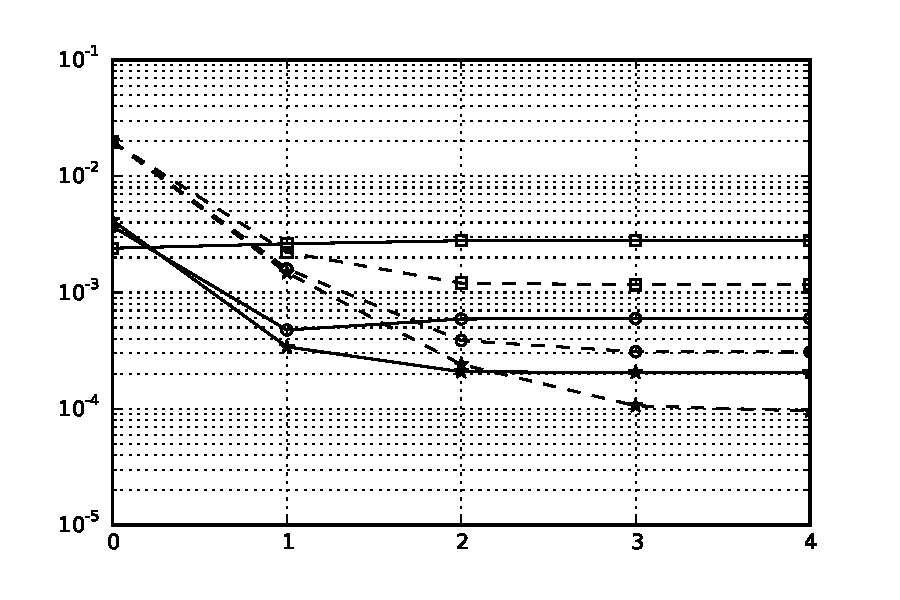
\includegraphics[width=0.8\textwidth]{UQAP/convergence1D}
  \bicaption[Fig:1]{例一:$\rho$均值的误差(实线)和标准差的误差(虚线)与gPC阶数的关系。这里$\eps = 10^{-8}$: $\Delta x = 0.04$(方形),$\Delta x = 0.02$(圆圈),$\Delta x = 0.01$(星号)。}{例一:$\rho$均值的误差(实线)和标准差的误差(虚线)与gPC阶数的关系。这里$\eps = 10^{-8}$: $\Delta x = 0.04$(方形),$\Delta x = 0.02$(圆圈),$\Delta x = 0.01$(星)。}{Fig}{Example 1. Errors of the mean (solid line) and standard deviation (dash line) of $\rho$ with respect to the gPC order at $\eps = 10^{-8}$: $\Delta x = 0.04$ (squares), $\Delta x = 0.02$ (circles), $\Delta x = 0.01$ (stars).}
\end{figure}

在图\ref{Fig:1}中,我们绘制了gPC数值解的均值和标准偏差的误差在$t = 0.01$与gPC阶数关系。三组结果包括:$\Delta x = 0.04$(正方形),$\Delta x = 0.02$(圆圈),$\Delta x = 0.01$(星)。这里$\Delta t = 0.0002 / 3$。可以看到,误差随着$N$增大快速衰减,然后在空间离散误差占优势变缓。很明显,即使$\eps = 10^{-8}$,由gPC展开导致的误差在$M = 4$时就可以被忽略。解的均值和标准偏差的曲线分别显示在图\ref{Fig:2}的左边和右边。

图\ref{Fig:6}中我们还绘制了的通量$vf$的平均值和标准偏差的曲线。在这里我们观察到gPC-SG方法和配点法以及参考解(\ref{limiting solution})之间良好的一致性。
\begin{figure}[htbp]
  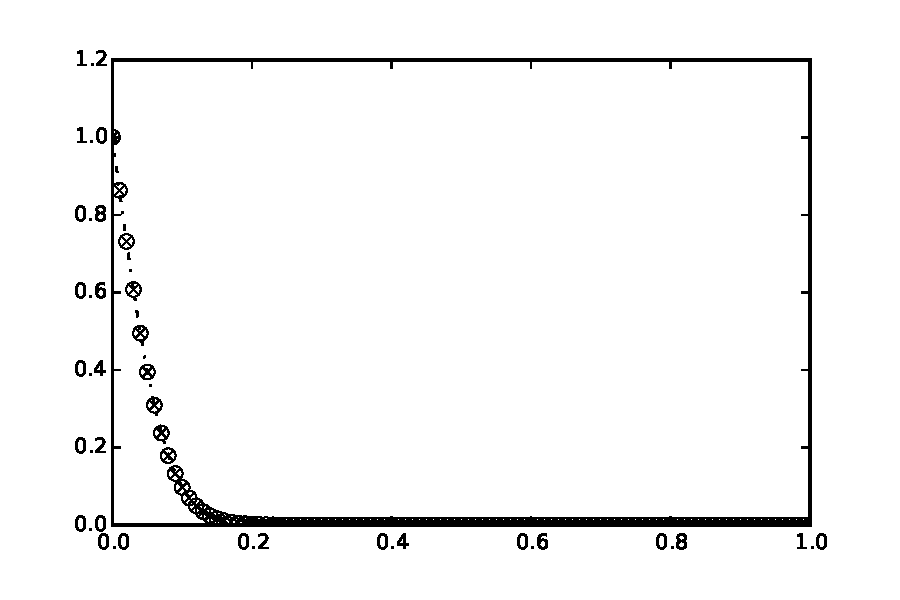
\includegraphics[width=0.5\textwidth]{UQAP/mean1D}
  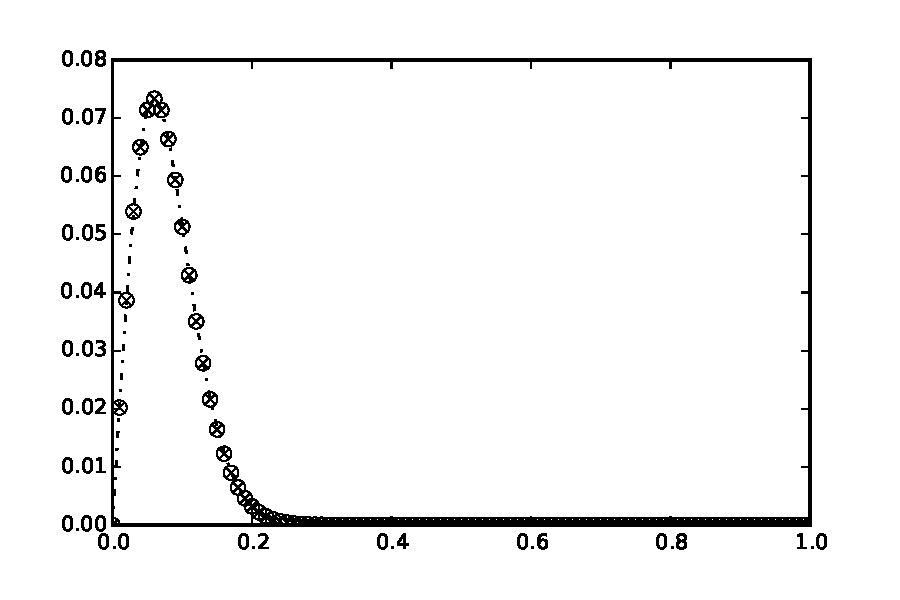
\includegraphics[width=0.5\textwidth]{UQAP/std1D}
  \bicaption[Fig:2]{例一:$\rho$的均值(左)和标准差(右)。$ \eps = 10 ^ {-8}$,gPC-SG方法$M = 4$(圆圈),配点法(叉)和极限解析解(\ref{limiting solution})。}{例一:$\rho$的均值(左边)和标准差(右边)。$ \eps = 10 ^ {-8}$,gPC-SG方法$M = 4$(圆圈),配点法(叉)和极限解析解(\ref{limiting solution})。}{Fig}{Example 1. The mean (left) and standard deviation (right) of $\rho$ at $\eps=10^{-8}$, obtained by the gPC Galerkin at order $M=4$ (circles), the stochastic collocation method (crosses), and the limiting analytical solution~(\ref{limiting solution}).}
\end{figure}
\begin{figure}[htbp]
  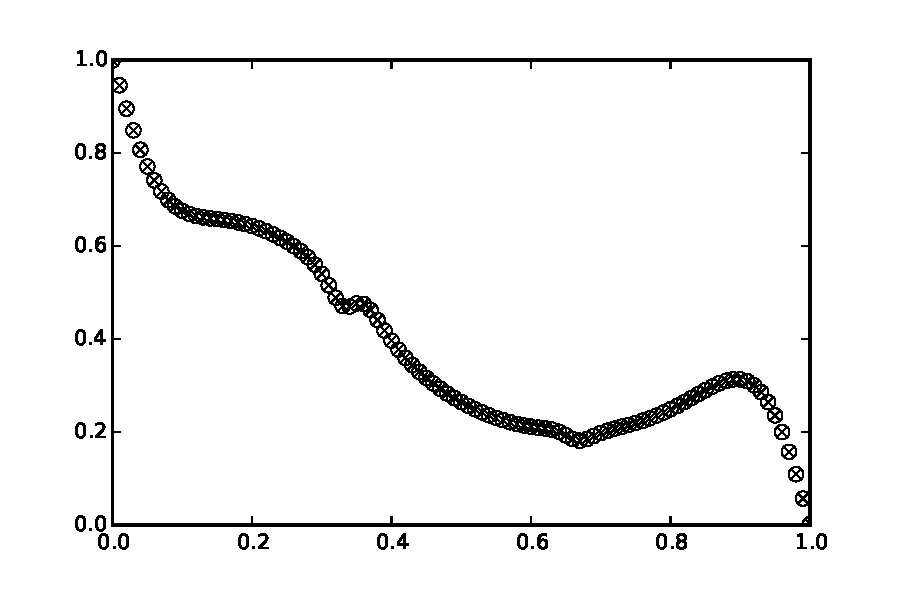
\includegraphics[width=0.5\textwidth]{UQAP/mean1D001}
  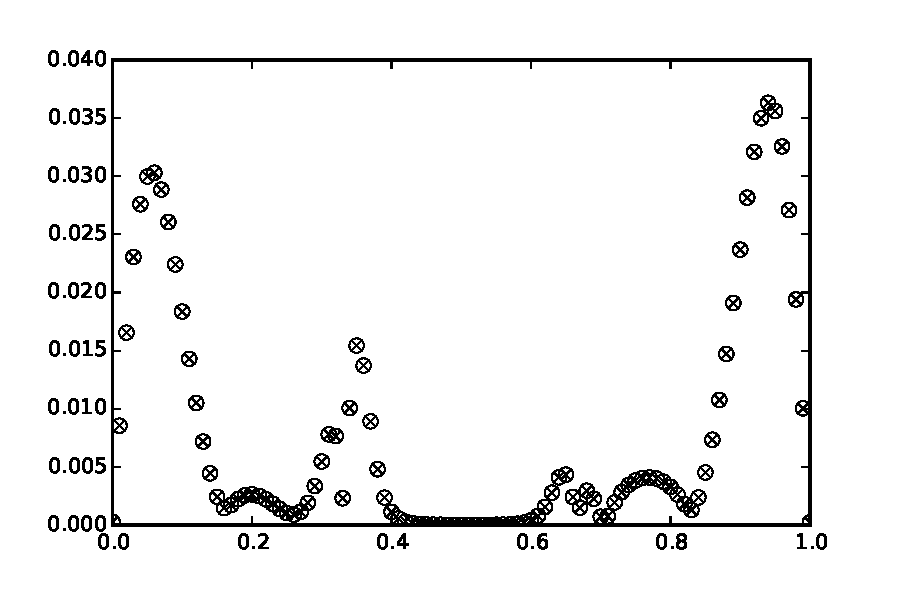
\includegraphics[width=0.5\textwidth]{UQAP/std1D001}
  \bicaption[Fig:6]{例一:均值(左)和标准差(右),gPC-SG方法(圆圈)和配点法(叉),$t=0.01$。}{例一:均值(左)和标准差(右),gPC-SG方法(圆圈)和配点法(叉),$t=0.01$。}{Fig}{Example 1. The mean (left) and standard deviation (right) obtained by gPC-Galerkin (circle) and collocation method (cross) at time $t=0.01$}
\end{figure}
\begin{figure}[htbp]  
  \centering
  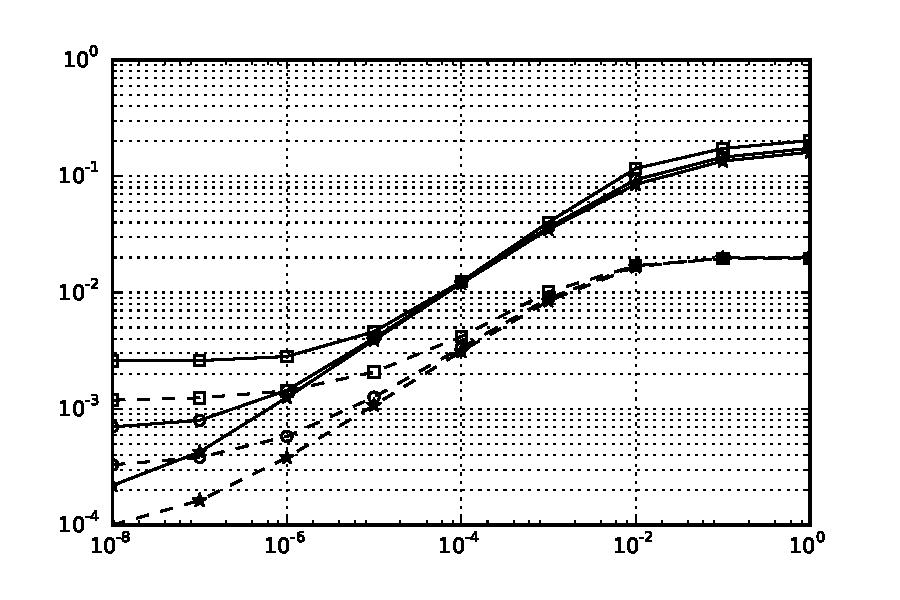
\includegraphics[width=0.8\textwidth]{UQAP/EPS_1D}
  \bicaption[Fig:3]{例一:两种解:解析解(\ref{limiting solution})和四阶gPC-SG方法,$\rho$的均值误差(实线)和标准差误差(虚线)与$\eps^2$的关系。$\Delta x = 0.04$ (方形), $\Delta x = 0.02$ (圆圈) and $\Delta x = 0.01$ (星)。}{例一:两种解:解析解(\ref{limiting solution})和四阶gPC-SG方法,$\rho$的均值误差(实线)和标准差误差(虚线)与$\eps^2$的关系。$\Delta x = 0.04$ (方形), $\Delta x = 0.02$ (圆圈) and $\Delta x = 0.01$ (星)。}{Fig}{Example 1. Differences in the mean (solid line) and standard deviation (dash line) of $\rho$ with respect to $\eps^2$, between the limiting analytical solution(\ref{limiting solution}) and the 4th-order gPC solution with $\Delta x = 0.04$ (squares), $\Delta x = 0.02$ (circles) and $\Delta x = 0.01$ (stars).}
\end{figure}

在图\ref{Fig:3}中,我们检查由四阶gPC-SG方法获得的解在$t = 0.01$时$\Delta x = 0.01$,$\Delta t = \Delta x^2/12$与极限方程解析解(\ref{limiting solution})的误差。正如预期,在数值误差占主导之前当$\eps^2$变小的时候误差会随之变小。
\subsection{例二:混合尺度}
在这个测试中,我们仍然令$\sigma = 2 + z$。考虑如果$\eps>0$也在一个较大的混合尺度上依赖于空间变量:
\begin{equation}
\eps(x)=10^{-3}+\frac{1}{2}[\tanh(6.5-11x)+\tanh(11x-4.5)]
\end{equation}
并光滑地从$O(10^{-3})$变到$O(1)$,如图\ref{Fig:7}。这种情况下会验证我们格式在混合多尺度下的适应能力,尤其是关于$\eps$的一致收敛性。
\begin{figure}[htbp]
  \centering
  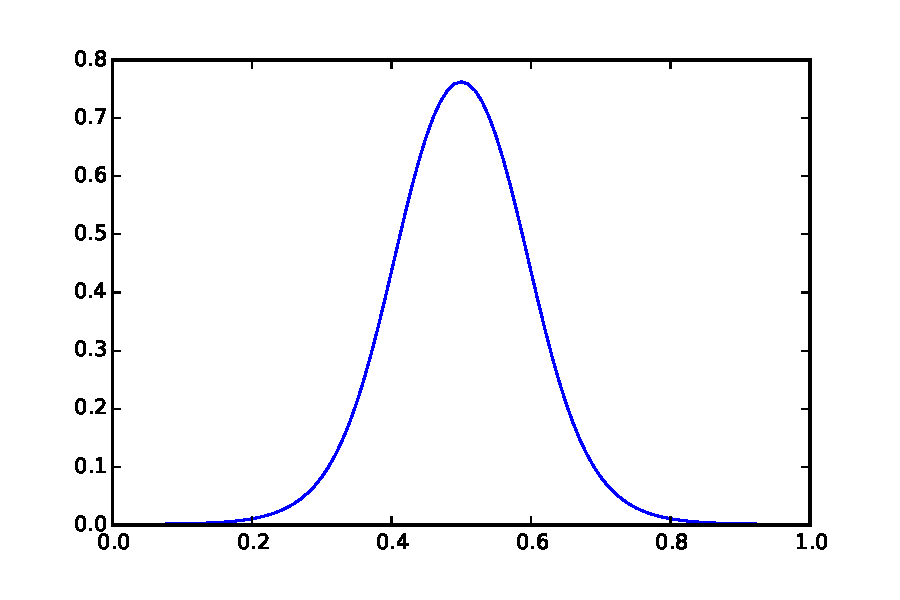
\includegraphics[width=0.8\textwidth]{UQAP/epsilon}
  \bicaption[Fig:7]{$\eps(x)$}{$\eps(x)$}{Fig}{$\eps(x)$}
\end{figure}

为了使质量仍然守恒,正确的线性输运方程为如下的形式,
\begin{equation}
  \dt f + v \dx\Big(\frac{1}{\varepsilon(x)} f\Big) = \frac{\sigma}{\eps^2(x)}{\cal L} f - \sigma^a f + S, \qquad \sigma(x, z) \ge \sigma_{\text{min}} > 0,
\end{equation}
那么micro-macro分解(\ref{eq-mM})修改为
\begin{subequations}
  \begin{align}
    & \dt \rho + \dx\av{vg} = -\sigma^a \rho + S ,  \\
    & \dt g + \frac{1}{\eps(x)} (I-\av{.}) (v\dx g) = -\frac{\sigma(z)}{\eps^2(x)}g  - \sigma^a g - \frac{1}{\eps(x)}v \dx\Big(\frac{1}{\varepsilon(x)}\rho\Big).
  \end{align}
\end{subequations}
可以发现只有最后一项发生了变化。对于极限方程(\ref{eq-diff1}),也需要修改为
\begin{equation}
  \dt \rho =  \partial_{x} (\kappa(z)  \partial_{x}\rho) - \dx(\kappa(z)a(x)\rho)-\sigma^a(z) \rho +S,
\end{equation}
其中我们假设
\begin{equation}
  a(x) =\lim\limits_{\varepsilon\rightarrow 0}\frac{\varepsilon'(x)}{\varepsilon(x)},
\end{equation}
存在。对于相应的数值格式,我们也只需要把(\ref{eq-schg})中的最后一项
\begin{equation}
  -\frac{1}{\eps^2}v\frac{\hrhonip-\hrhoni}{\Dx}
\end{equation}
替换为
\begin{equation}
   -\frac{1}{\eps(x_{i+1/2})}v\Bigg(\frac{\hrhonip}{\eps(x_{i+1})}-\frac{\hrhoni}{\eps(x_i)}\Bigg)\frac{1}{\Dx}.ß
\end{equation}

初值为
\begin{equation}\label{eg2-ini1}
f_{\text{in}}(x,v,z)=\frac{\rho_0}{2}\big [\exp\big(-(\frac{v-0.75}{T_0})^2\big)+\exp\big(-(\frac{v+0.75}{T_0})^2\big)\big ]
\end{equation}
其中
\begin{equation}\label{eg2-ini2}
\rho_0(x)=\frac{2+\sin(2\pi x)}{2},\quad T_0(x)=\frac{5+2\cos(2\pi x)}{20}.
\end{equation}

参考解是由配点法(30样本)得到。相关参数如下:网格空间$\Delta x = 0.01$,时间$\Delta t = \Delta x^2/3$。我们用五阶gPC-SG方法分别演化到时刻$t=0.005$,$t=0.01$, $t=0.05$, $t=0.1$。对于$v$方向的积分,我们使用30个点的高斯积分。

图\ref{Fig:8}显示了均值和标准差的$\ell^2$误差与gPC阶数的关系,可以看出收敛的非常快(谱收敛)。
\begin{figure}[htbp]
  \centering
  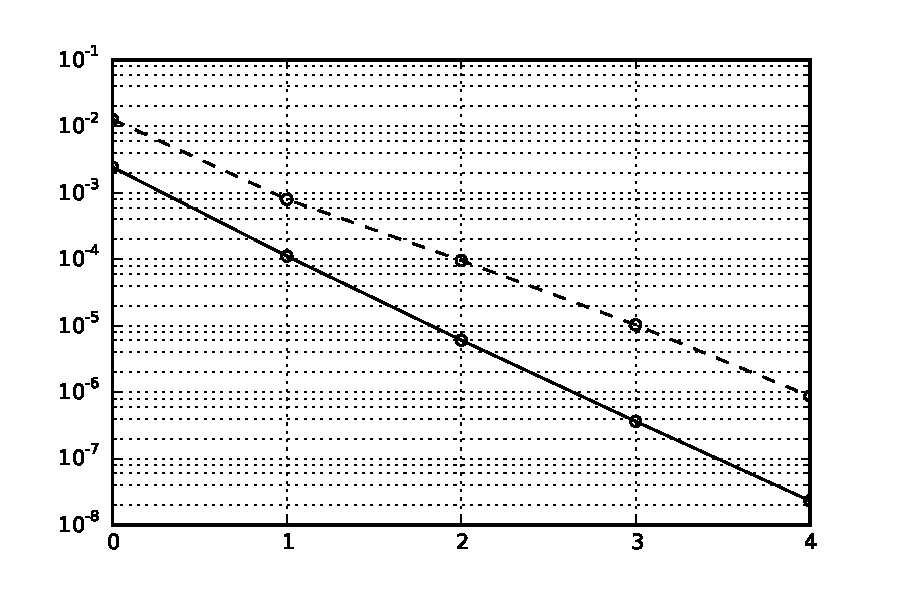
\includegraphics[width=0.8\textwidth]{UQAP/convergence1Deps}
  \bicaption[Fig:8]{例二:均值(实线)和标准差(虚线)的$\ell^2$误差与gPC阶数的关系}{例二:均值(实线)和标准差(虚线)的$\ell^2$误差与gPC阶数的关系}{Fig}{Example 2 with initial data(\ref{eg2-ini1})--(\ref{eg2-ini2}). The $\ell^2$ error of mean and standard deviation (dash line) with respect to gPC order. }
\end{figure}

\subsection{例三:随机初值}
接下来我们在初值上加入随机性($\sigma=2+z$仍然随机)。
\begin{equation}
f(0,x,v,z) = f(0,x,v)+0.2z
\end{equation}
其中$f(x,v,0)$和(\ref{eg2-ini1})中一样。这次$\Dx=0.01$,$\Delta t = \Delta x^2/12$以及最终时间$T=0.01$。首先我们测试流体极限$\varepsilon=10^{-8}$,如图\ref{Fig:9}。
\begin{figure}[htbp]
  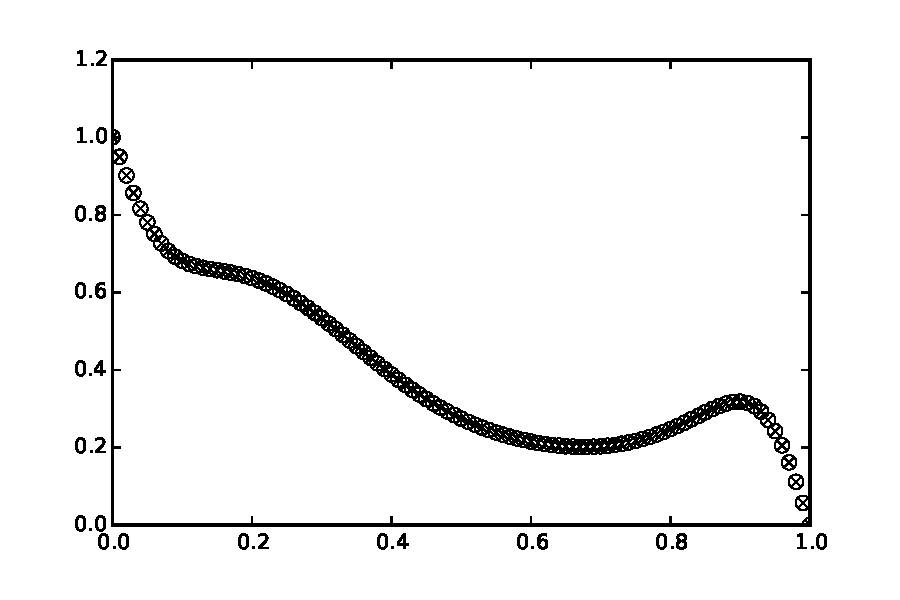
\includegraphics[width=0.5\textwidth]{UQAP/mean1Dir}
  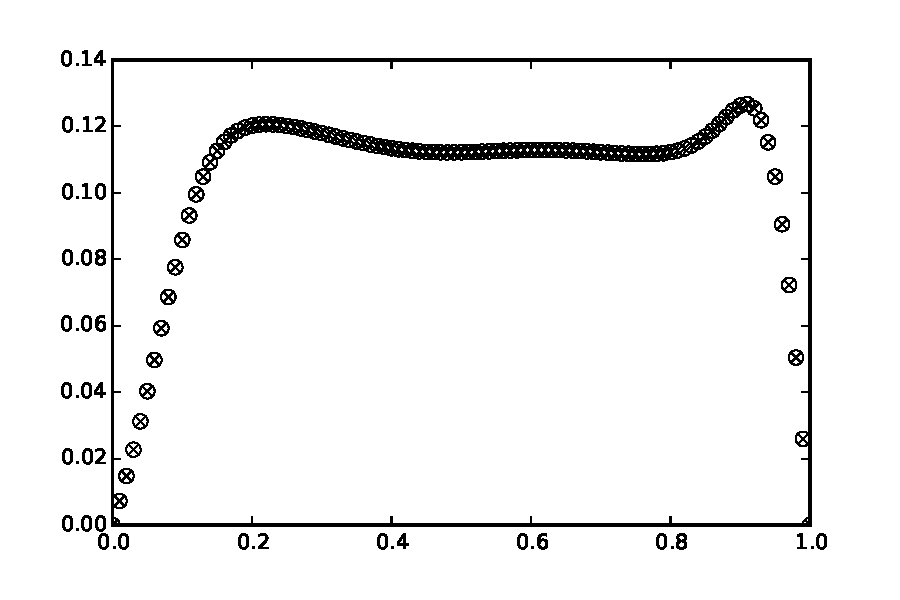
\includegraphics[width=0.5\textwidth]{UQAP/std1Dir}
  \bicaption[Fig:9]{例三:均值(左)和标准差(右),gPC-SG方法(圆圈)和配点法(叉),$t=0.1$,$\varepsilon=10^{-8}$。}{例三:均值(左)和标准差(右),gPC-SG方法(圆圈)和配点法(叉),$t=0.1$,$\varepsilon=10^{-8}$。}{Fig}{Example 3. The mean (left) and standard deviation (right) obtained by gPC-Galerkin (circle) and collocation method (cross) at time $t=0.1$, $\varepsilon=10^{-8}$.}
\end{figure}
接下来我们测试$\varepsilon=1$,如图\ref{Fig:10}。
\begin{figure}[htbp]
  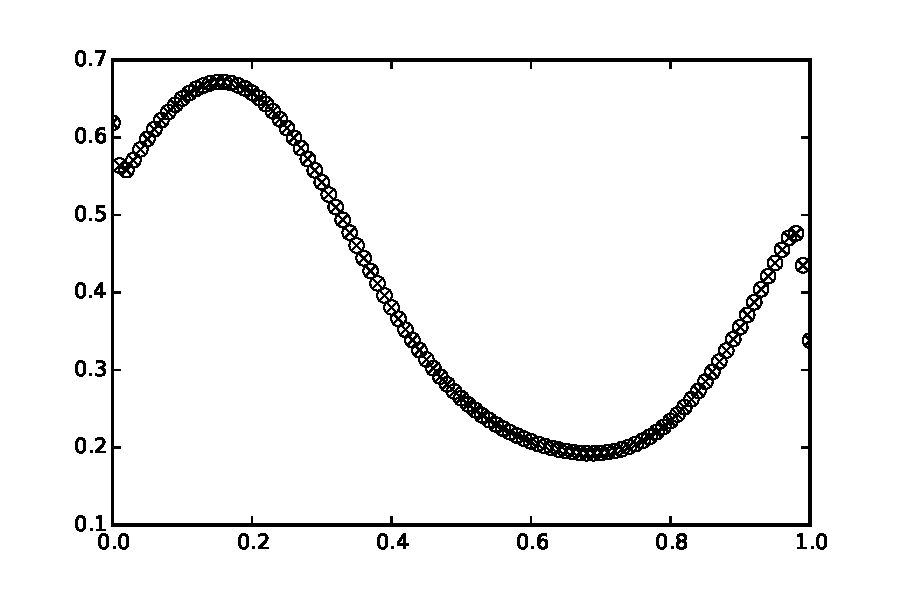
\includegraphics[width=0.5\textwidth]{UQAP/mean1DirO1}
  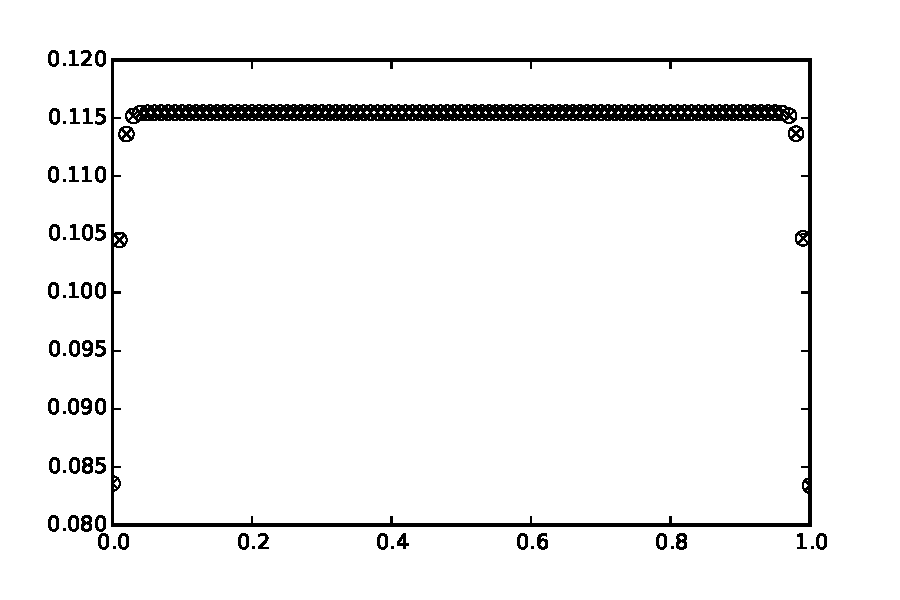
\includegraphics[width=0.5\textwidth]{UQAP/std1DirO1}
  \bicaption[Fig:10]{例三:均值(左)和标准差(右),gPC-SG方法(圆圈)和配点法(叉),$t=0.1$, $\varepsilon=1$。}{例三:均值(左)和标准差(右),gPC-SG方法(圆圈)和配点法(叉),$t=0.1$, $\varepsilon=1$。}{Fig}{Example 3. The mean (left) and standard deviation (right) obtained by gPC-Galerkin (circle) and collocation method (cross) at time $t=0.1$, $\varepsilon=1$}
  % \label{Fig:10}
\end{figure}
可以看到两种方法吻合度很高。

\subsection{例四:随机边界条件}
这个例子中,我们在边界条件中加入随机性:
\begin{equation}
f_L(t,v,z) = 2 + z,\quad f_R(t,v,z) = 1 + z.
\end{equation}
我们也测试了当$\varepsilon=10^{-8}$和$\varepsilon=10$两种情况,如图\ref{Fig:11}和图\ref{Fig:12},同样的gPC-SG方法和参考解高度吻合。
\begin{figure}[htbp]
  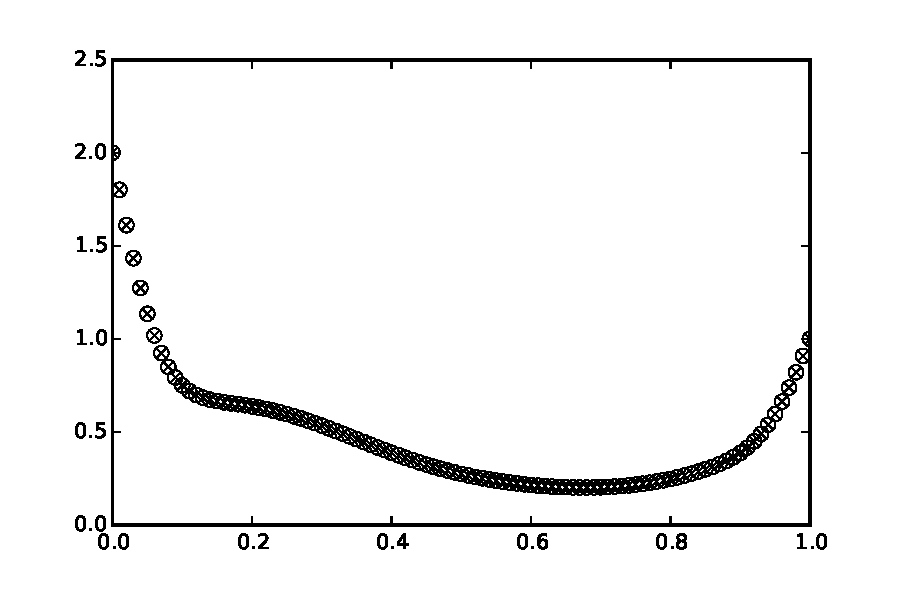
\includegraphics[width=0.5\textwidth]{UQAP/mean1Dbr}
  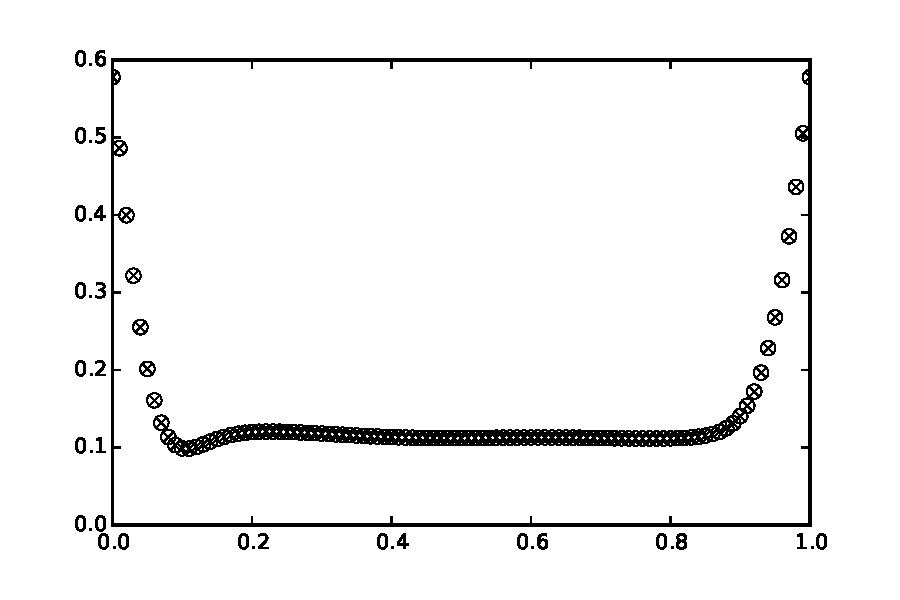
\includegraphics[width=0.5\textwidth]{UQAP/std1Dbr}
  \bicaption[Fig:11]{例四:均值(左)和标准差(右),gPC-SG方法(圆圈)和配点法(叉),$t=0.1$, $\varepsilon=10^{-8}$。}{例四:均值(左)和标准差(右),gPC-SG方法(圆圈)和配点法(叉),$t=0.1$, $\varepsilon=10^{-8}$。}{Fig}{Example 4. The mean (left) and standard deviation (right) obtained by gPC-Galerkin (circle) and collocation method (cross) at time $t=0.1$, $\varepsilon=10^{-8}$}
\end{figure}
\begin{figure}[htbp]
  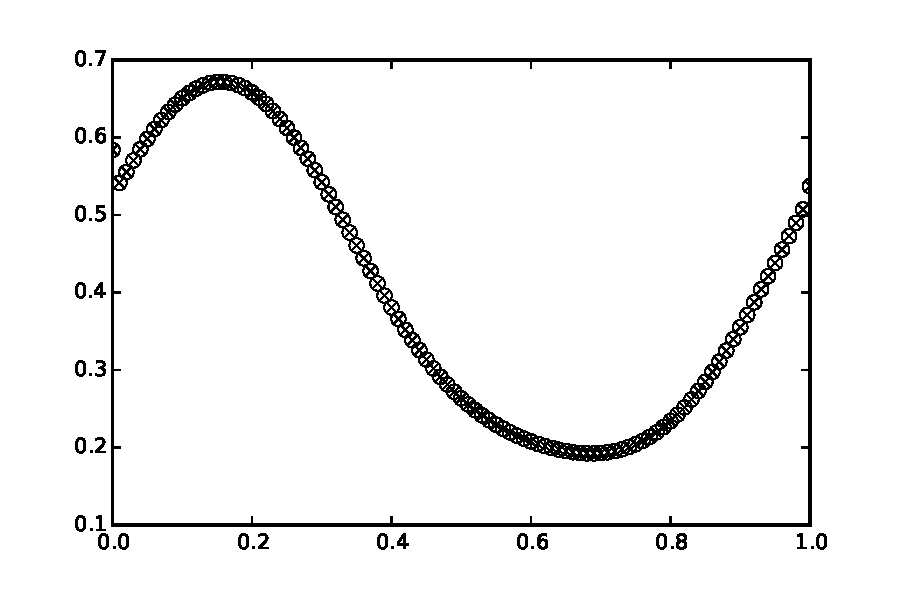
\includegraphics[width=0.5\textwidth]{UQAP/mean1DbrO10}
  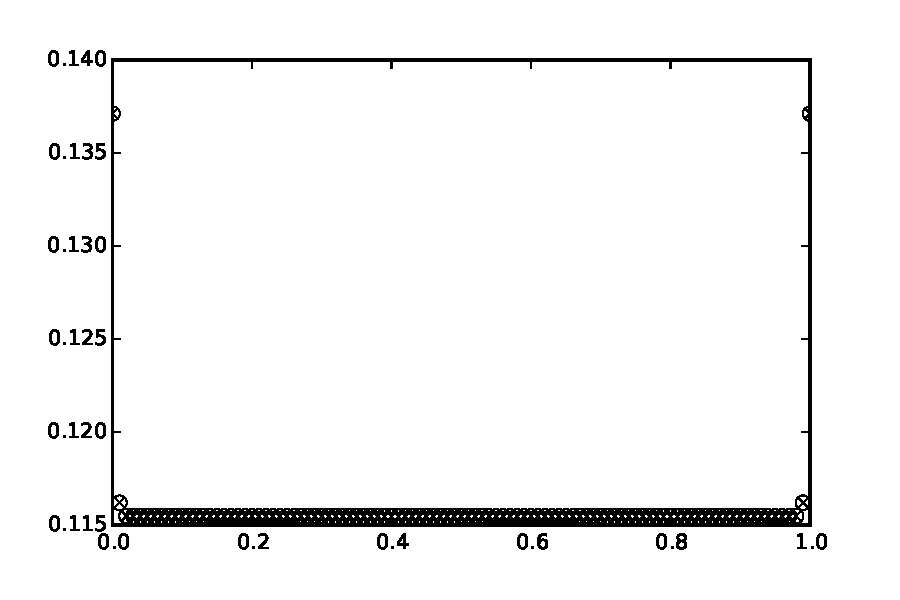
\includegraphics[width=0.5\textwidth]{UQAP/std1DbrO10}
  \bicaption[Fig:12]{例四:均值(左)和标准差(右),gPC-SG方法(圆圈)和配点法(叉),$t=0.1$, $\varepsilon=10$。}{例四:均值(左)和标准差(右),gPC-SG方法(圆圈)和配点法(叉),$t=0.1$, $\varepsilon=10$。}{Fig}{Example 4. The mean (left) and standard deviation (right) obtained by gPC-Galerkin (circle) and collocation method (cross) at time $t=0.1$, $\varepsilon=10$}
\end{figure}


\subsection{例五:二维随机空间}
最后,我们来考察具有如下形式的二维随机场:
\begin{equation}
  \sigma(x,z_1,z_2) = 1 - \frac{\sigma z_1}{\pi^2}\cos(2\pi x) - \frac{\sigma z_2}{4\pi^2}\cos(4\pi x)
\end{equation}
% where we set $\sigma=4$ and $z_1, z_2$ are both uniformly distributed in $(-1,1)$. The mean and standard deviation of the solution $\rho$ at $t=0.01$ obtained by the 5th-order gPC Galerkin with $\Delta x = 0.025$, $\Delta t = 0.0002/3$ are shown in Figure\ref{Fig:4}. We then use the high-order stochastic collocation  method over 40$\times$40 Gauss-Legendre quadrature points to compute the reference mean and standard deviation of the solutions. In Figure\ref{Fig:5}, we show the errors of the mean (solid lines) and standard deviation (dash lines) of $\rho$ with respect to the order of gPC expansion. The fast spectral convergence of the errors can be clearly seen.

其中我们设置$\sigma = 4$和$z_1,z_2$为均匀分布在$(-1,1)$上的随机变量。由$\Delta x = 0.025$,$\Delta t = 0.0002 / 3$的五阶gPC-SG方法得到在$t = 0.01$的解$\rho$的均值和标准偏差见图\ref{Fig:4}。然后我们使用高阶配点法(40$\times$40高斯 - 勒让德积分点)来计算解的参考解的均值和标准差。在图\ref{Fig:5}中,我们画出$\rho$的均值(实线)和标准差(虚线)的误差与gPC阶数的关系。可以清楚地看到误差的快速谱收敛。
\begin{figure}[H]  
  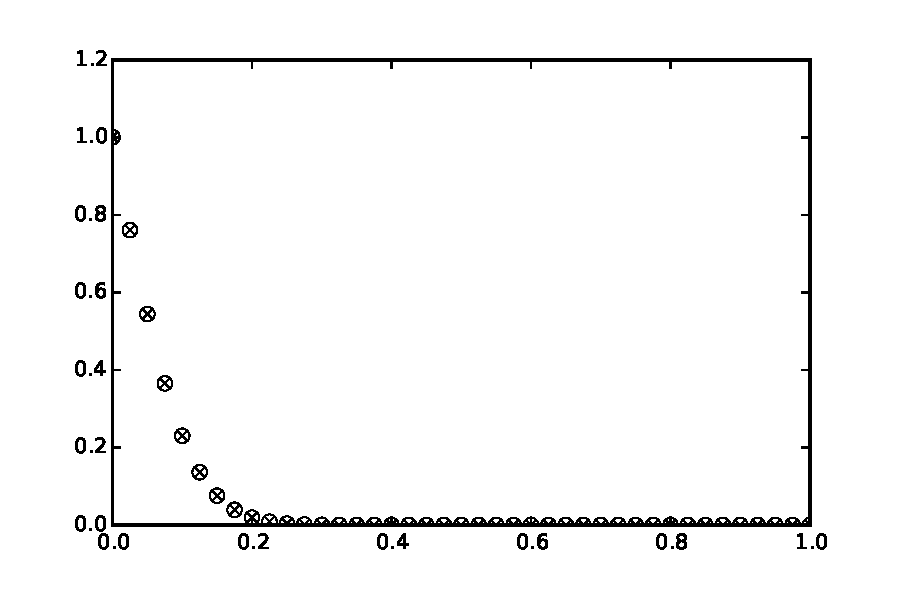
\includegraphics[width=0.5\textwidth]{UQAP/mean2D}
  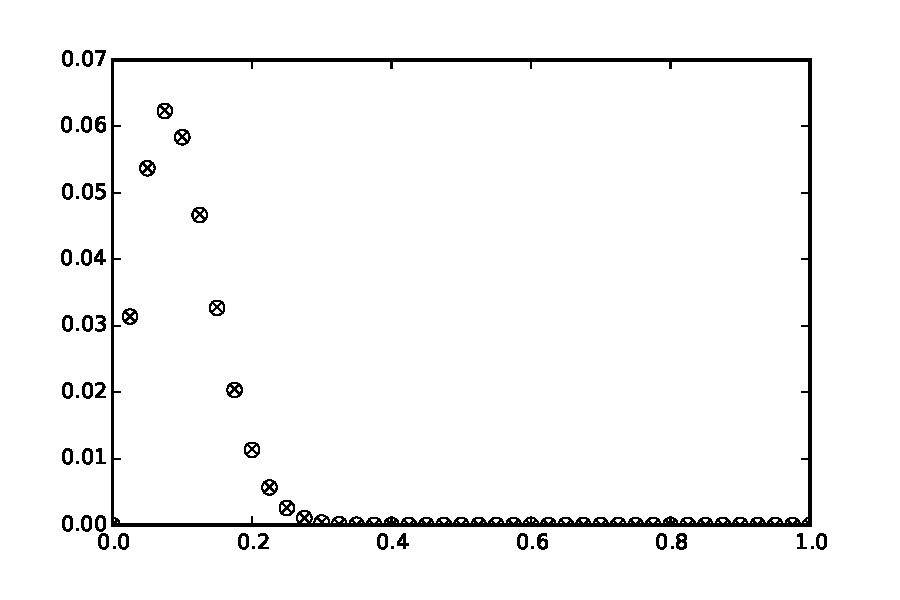
\includegraphics[width=0.5\textwidth]{UQAP/std2D}
  \bicaption[Fig:4]{均值(左)和标准差(右),五阶gPC-SG方法(圆圈)和配点法(叉),二维随机变量。}{均值(左)和标准差(右),五阶gPC-SG方法(圆圈)和配点法(叉),二维随机变量。}{Fig}{The mean (left) and standard deviation (right) of $\rho$ at $\eps = 10^{-8}$, obtained by 5th-order gPC Galerkin (circles) and the stochastic collocation method (crosses). The random input has dimension $d=2$.}
\end{figure}
\begin{figure}[H]  
  \centering
  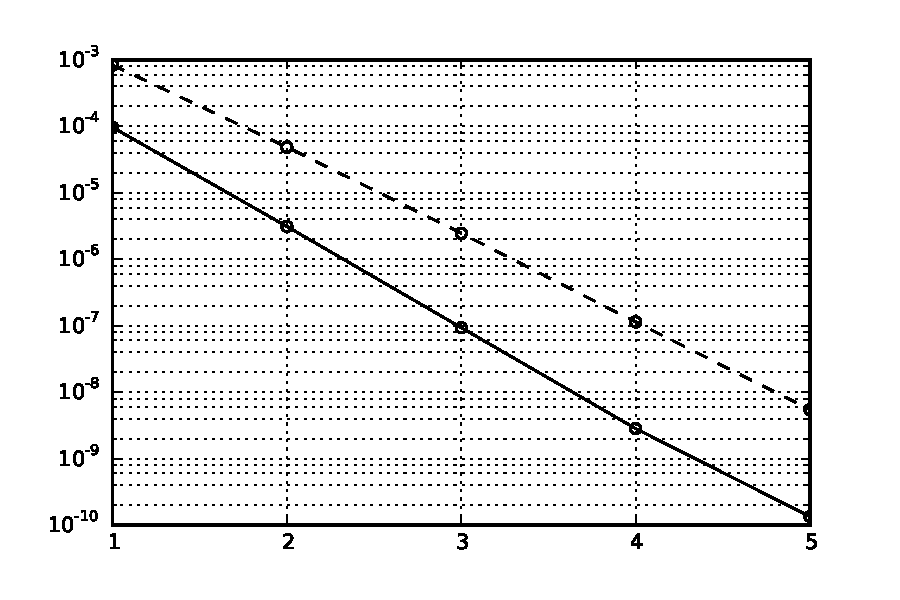
\includegraphics[width=0.8\textwidth]{UQAP/convergence2D}
  \bicaption[Fig:5]{$\rho$的均值误差(实线)和标准差误差(虚线)与gPC-SG阶数的关系,二维随机变量。}{$\rho$的均值误差(实线)和标准差误差(虚线)与gPC-SG阶数的关系,二维随机变量。}{Fig}{Errors of the mean (solid line) and standard deviation (dash line) of $\rho$ with respect to gPC order, with the $d=2$ dimensional random input.}
\end{figure}


%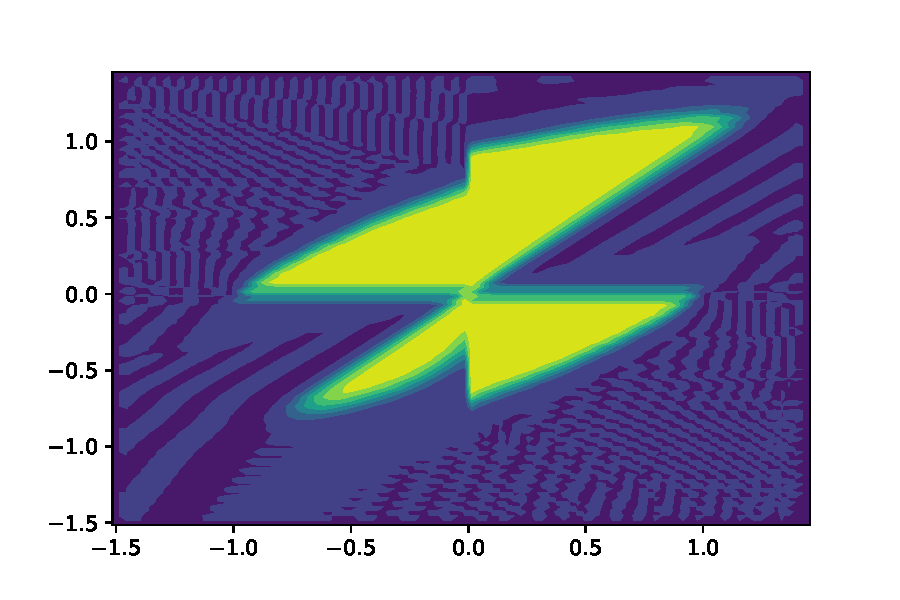
\includegraphics[scale=.8]{mean.pdf}

%\includegraphics[scale=.8]{deviation.pdf}

%\includegraphics[scale=.8]{err_gpc_order_1.pdf}


%\includegraphics[scale=.8]{error_eps.pdf}

\section{本章总结与展望} \label{sec:conl}

在本章中,我们建立了随机伽辽金方法对带有随机散射系数的线性输运方程关于克努森数一致的谱精度分析,从而允许我们证明该方法具有随机渐近保持性质(s-AP)。对于基于micro-macro分解的全离散格式,我们证明了一致的稳定性结果。这是首次有人证明了关于这类问题的一致性结果。

关于一致性的分析在带有多尺度与不确定性的问题中非常重要。我们的分析对于线性问题具有一般的指导意义,进而可以推广到更多的kinetic方程或其他方程上去。而对于非线性的问题,仍然非常困难,将作为未来的研究的内容。


% \bibliographystyle{plain}
% \bibliography{UQAP_bibtex}

% \end{document}

% ==============

% We proceed in five short steps.

% \noindent {\it Step 1.} \\
% Here we derive a first energy relation. With the finite difference operators defined
% in(\ref{eq-diff_onesided})--(\ref{eq-diff_centered2}), our scheme can
% be written in the following compact form:
% \begin{subequations}\label{eq-cscheme}
%   \begin{align}
% & \frac{\hrhonpi-\hrhoni}{\Dt} + \Dnot\av{v\hgnp_i} = 0 \label{eq-srho}
% \\
% & \frac{\hgnpi-\hgni}{\Dt} + \frac{1}{\eps} (I-\av{.})
% \left(v^+\Dm+v^-\Dp\right)\hgni = - \frac{\Sigma}{\eps^2} \hgnpi
% - \frac{1}{\eps^2}v\,\dnot \hrhon_{i+\half}.\label{eq-sg}
%   \end{align}
% \end{subequations}


% We define the energy of system(\ref{eq-mM}) as $\int_\R \hat \rho^2 \, \diff x +
% \eps^2 \int \av{\hat g^2} \, \diff x$. It is clear that our scheme can be proved
% to be stable if the energy at time $n+1$ can be controlled by the
% energy at time $n$. Consequently, we first multiply(\ref{eq-srho}) by
% $\hrhonpi$, then we take the sum over $i\in\Z$, and finally, we use
% the standard equality $a(a-b)=\half(a^2-b^2+|a-b|^2)$ to get:
% \begin{subequations}
% \begin{equation}  \label{eq-Erho}
% \frac{1}{2\Dt} \left(  \rnorm{\hrhonp}^2- \rnorm{\hrhon}^2+\rnorm{\hrhonp-\hrhon}^2\right)
% + \sumi \hrhonpi\Dnot\av{v\hgnp_i}\Dx = 0.
% \end{equation}
% Second, we multiply(\ref{eq-sg}) by $\hgnpi$, we take the velocity
% average, we sum over $i\in \Z$, and we get:
% \begin{equation}  \label{eq-Eg}
% \begin{split}
% & \frac{1}{2\Dt} \left( \gnorm{\hgnp}^2-\gnorm{\hgn}^2 + \gnorm{\hgnp-\hgn}^2  \right)
% + \frac{1}{\eps}\innerp{\hgnp}{(I-\av{.})\left(v^+\Dm+v^-\Dp\right)\hgn} \\
% &  = - \frac1{\eps^2}  \langle \hgnp, {\hat \sigma} \hgnp \rangle - \frac{1}{\eps^2}\sumi \av{v\hgnpi}\dnot \hrhon_{i+\half}\Dx.
% \end{split}
% \end{equation}
% \end{subequations}
% $$
%    \langle \hgnp, \Sigma \hgnp \rangle \ge \sigma_m \gnorm{\hgnp}^2
% $$
% Now we use proposition\ref{prop:gav}: since $\av{\hgnpi}=0$ for every
% $i$, a simple expansion of the inner product of(\ref{eq-Eg}) shows
% that it can be reduced to:
% \begin{equation}  \label{eq-Innp}
% \begin{split}
% & \innerp{\hgnp}{(I-\av{.})\left(v^+\Dm+v^-\Dp\right)\hgn}   \\
% & =  \innerp{\hgnp}{\left(v^+\Dm+v^-\Dp\right)\hgn}
% -  \sumi \av{\hgnpi}\av{\left(v^+\Dm+v^-\Dp\right)\hgni}\Dx \\
% & = \innerp{\hgnp}{\left(v^+\Dm+v^-\Dp\right)\hgn}.
% \end{split}
% \end{equation}
% Consequently, we add up(\ref{eq-Erho}) and $\eps^2$
% times(\ref{eq-Eg}), then we use(\ref{eq-Innp}) and
% the discrete integration by parts of lemma\ref{lemma:intbp} to get our preliminary energy relation:
% \begin{equation}  \label{eq-ener}
% \begin{split}
% & \frac{1}{2\Dt} \left(  \rnorm{\hrhonp}^2-\rnorm{\hrhon}^2+\rnorm{\hrhonp-\hrhon}^2\right)
% + \sumi \hrhonpi\Dnot\av{v\hgnp_i}\Dx \\
% & + \frac{\eps^2}{2\Dt} \left( \gnorm{\hgnp}^2-\gnorm{\hgn}^2 +
%   \gnorm{\hgnp-\hgn}^2  \right) + \eps
% \innerp{\hgnp}{\left(v^+\Dm+v^-\Dp\right)\hgn} \\
% & \le  -\sigma_m \gnorm{\hgnp}^2 + \sumi \av{v\Dnot\hgnp_i} \hrhoni\Dx.
% \end{split}
% \end{equation}

% \bigskip
% \noindent {\it Step 2.} \\
% In this step, we show how the $\hrhonp-\hrhon$ term can be eliminated
% in(\ref{eq-ener}). First, it is useful to write $\hrhoni$ in the
% right-hand side of(\ref{eq-ener}) as $(\hrhoni-\hrhonpi)+\hrhonpi$:
% indeed, the terms $\sumi \hrhonpi\Dnot\av{v\hgnp_i}$ and $\sumi
% \av{v\Dnot\hgnp_i} \hrhonpi$ in the left and right-hand sides cancel
% out and we obtain:
% \begin{equation}  \label{eq-enerbis}
% \begin{split}
% & \frac{1}{2\Dt} \left(  \rnorm{\hrhonp}^2-\rnorm{\hrhon}^2+\rnorm{\hrhonp-\hrhon}^2\right) \\
% & + \frac{\eps^2}{2\Dt} \left( \gnorm{\hgnp}^2-\gnorm{\hgn}^2 +
%   \gnorm{\hgnp-\hgn}^2  \right) + \eps��
% \innerp{\hgnp}{\left(v^+\Dm+v^-\Dp\right)\hgn} \\
% & \le  -\sigma_m \gnorm{\hgnp}^2 + \sumi \av{v\Dnot\hgnp_i} (\hrhoni-\hrhonpi)\Dx.��
% \end{split}
% \end{equation}
% Now, we use
% the following Young inequality:
% \begin{equation}  \label{eq-Yrho}
% \sumi \av{v\Dnot\hgnp_i}(\hrhoni-\hrhonpi)\Dx \leq \alpha \rnorm{\hrhonp-\hrhon}^2
% +\frac{1}{4\alpha}\sumi\av{v\Dnot\hgnp_i}^2\Dx.
% \end{equation}

%  the $\hrhonp-\hrhon$ terms cancel out in(\ref{eq-enerbis}) if $\alpha=\frac{1}{2\Dt}$
% and we get
% \begin{equation}  \label{eq-fener}
% \begin{split}
% & \frac{1}{2\Dt} \left(  \rnorm{\hrhonp}^2-\rnorm{\hrhon}^2\right)
% + \frac{\eps^2}{2\Dt} \left( \gnorm{\hgnp}^2-\gnorm{\hgn}^2 +  \gnorm{\hgnp-\hgn}^2  \right) \\
% & + \eps \innerp{\hgnp}{\left(v^+\Dm+v^-\Dp\right)\hgn} \leq
% -\sigma_m \gnorm{\hgnp}^2 +\frac{\Dt}{2}\sumi\av{v\Dnot\hgnpi}^2\Dx.
% \end{split}
% \end{equation}


% \bigskip
% \noindent {\it Step 3.} \\
% Here, we work on the inner product of(\ref{eq-fener}) to show that
% the $\hgnp-\hgn$ terms can also be eliminated. First, we insert $\hgnp$
% in this inner product to get:
% \begin{equation}  \label{eq-vDgg1}
% \begin{split}
% & \innerp{\hgnp}{\left(v^+\Dm+v^-\Dp\right)\hgn}  \\
% & = \innerp{\hgnp}{\left(v^+\Dm+v^-\Dp\right)\hgnp}
%      + \innerp{\hgnp}{\left(v^+\Dm+v^-\Dp\right)(\hgn-\hgnp)} \\
% & = A+B,
% \end{split}
% \end{equation}
% and we rewrite terms $A$ and $B$ as follows. For $A$, we use the
% centered form of the upwind operator (lemma\ref{lemma:5}) and
% the discrete integration by parts of lemma\ref{lemma:intbp} to get:
% \begin{equation}\label{eq-vDgg2}
% \begin{split}
% A & = \innerp{\hgnp}{v\Dc\hgnp} -\frac{\Dx}{2} \innerp{\hgnp}{|v|\Dm\Dp\hgnp} \\
% &  = \frac{\Dx}{2} \innerp{\Dp\hgnp}{|v|\Dp\hgnp} \\
% & = \frac{\Dx}{2} \sumi \av{|v|\left(\Dp\hgnpi\right)^2}\Dx.
% \end{split}
% \end{equation}
% For $B$, we also use the discrete integration by parts of
% lemma\ref{lemma:intbp} to get:
% \begin{equation}\label{eq-vDgg3}
% \begin{split}
% B= -\innerp{\left(v^+\Dp+v^-\Dm\right)\hgnp}{\hgn-\hgnp}.
% \end{split}
% \end{equation}
% Then we apply the inequality of lemma\ref{lemma:3} to $B$ to get
% \begin{equation}  \label{eq-YB}
% |B|\leq \alpha \gnorm{\hgnp-\hgn}^2+\frac{1}{4\alpha}\gnorm{|v|\Dp\hgnp}^2.
% \end{equation}
% Therefore, using(\ref{eq-fener}),(\ref{eq-vDgg1}),(\ref{eq-vDgg2})
% and(\ref{eq-YB}), we see that the $\hgnp-\hgn$ terms cancel out
% in(\ref{eq-fener}) if $\alpha=\frac{\eps}{2\Dt}$, and we get
% \begin{equation}\label{eq-enera}
% \begin{split}
% & \frac{1}{2\Dt} \left(  \rnorm{\hrhonp}^2-\rnorm{\hrhon}^2\right)
% + \frac{\eps^2}{2\Dt} \left( \gnorm{\hgnp}^2-\gnorm{\hgn}^2 \right) \\
% & + \eps\frac{\Dx}{2} \sumi \av{|v|\left(\Dp\hgnpi\right)^2}\Dx
%   - \frac{\Dt}{2}\gnorm{|v|\Dp\hgnp}^2   \\
% & \leq   - \sigma_m \gnorm{\hgnp}^2 +\frac{\Dt}{2}\sumi\av{v\Dnot\hgnpi}^2\Dx.
% \end{split}
% \end{equation}

% \bigskip
% \noindent {\it Step 4.} \\
% Now, we show how all the $\Dp \hgnp$ and the $\Dnot \hgnp$ terms can be
% controlled by $\gnorm{\hgnp}$. First, note that the term
% $\frac{\Dt}{2}\gnorm{|v|\Dp\hgnp}^2$ of the left-hand side
% of(\ref{eq-enera}) can be estimated as follows:
% \begin{equation}\label{eq-majDg}
% \begin{split}
% \frac{\Dt}{2}\gnorm{|v|\Dp\hgnp}^2 & =  \frac{\Dt}{2} \sumi \av{|v|^2\left(\Dp\hgnpi\right)^2}\Dx \\
% & \leq \frac{\Dt}{2} \sumi \av{|v|\left(\Dp\hgnpi\right)^2}\Dx,
% \end{split}
% \end{equation}
% since $|v|\leq 1$. Moreover, using lemma\ref{lemma:2} and a change
% of indices shows that the
% last term of the right-hand side of(\ref{eq-enera}) satisfies
% \begin{equation}  \label{eq-majDnotg}
% \frac{\Dt}{2}\sumi\av{v\Dnot\hgnpi}^2\Dx \leq \frac{\Dt}{4}\sumi\av{|v|\left(\Dp\hgnpi\right)^2}\Dx.
% \end{equation}
% Finally, we use these two estimates in(\ref{eq-enera}) to obtain:
% \begin{equation}\label{eq-enerf}
% \begin{split}
% & \frac{1}{2\Dt} \left(  \rnorm{\hrhonp}^2-\rnorm{\hrhon}^2\right)
% + \frac{\eps^2}{2\Dt} \left( \gnorm{\hgnp}^2-\gnorm{\hgn}^2 \right)   \\
% & \leq  - \sigma_m\gnorm{\hgnp}^2 + \left(\frac{3\Dt}{4}- \eps\frac{\Dx}{2}\right) \sumi \av{|v|\left(\Dp\hgnpi\right)^2}\Dx.
% \end{split}
% \end{equation}
% Now, taking the positive part of the factor $(\frac{3\Dt}{4}- \eps\frac{\Dx}{2})$ of the
% right-hand side of(\ref{eq-enerf}), we have the estimate
% \begin{equation}\label{eq-enerfb}
% \begin{split}
%   \left(\frac{3\Dt}{4}- \eps\frac{\Dx}{2}\right) \sumi \av{|v|\left(\Dp\hgnpi\right)^2}\Dx
% & \leq   \left(\frac{3\Dt}{4}- \eps\frac{\Dx}{2}\right)^+ \sumi \av{\left(\Dp\hgnpi\right)^2}\Dx \\
% & \leq   \left(\frac{3\Dt}{4}- \eps\frac{\Dx}{2}\right)^+ \frac{4}{\Dx^2} \gnorm{\hgnp}^2,
% \end{split}
% \end{equation}
% where we have used $|v|\leq 1$ and the estimate of lemma\ref{lemma:estimDp}.


% \bigskip
% \noindent {\it Step 5.}  \\
% Finally, estimates(\ref{eq-enerf}) and(\ref{eq-enerfb}) show that
% \begin{equation*}
%    \frac{1}{2\Dt} \left(  \rnorm{\hrhonp}^2-\rnorm{\hrhon}^2\right)
% + \frac{\eps^2}{2\Dt} \left( \gnorm{\hgnp}^2-\gnorm{\hgn}^2 \right)
% \leq \left( \left(\frac{3\Dt}{4}- \eps\frac{\Dx}{2}\right)^+ \frac{4}{\Dx^2}-\sigma_m\right) \gnorm{\hgnp}^2.
% \end{equation*}
% This means that we have the final energy estimate
% \begin{equation*}
%   \rnorm{\hrhonp}^2+ \eps^2\gnorm{\hgnp}^2 \leq \rnorm{\hrhon}^2+ \eps^2\gnorm{\hgn}^2
% \end{equation*}
% if $\Dt$ is such that
% \begin{equation*}
%   \left(\frac{3\Dt}{4}- \eps\frac{\Dx}{2}\right)^+ \frac{4}{\Dx^2}\leq\sigma_m.
% \end{equation*}
% Since $\sigma_m > 0$, an equivalent condition is $(\frac{3\Dt}{4}- \eps\frac{\Dx}{2})
% \frac{4}{\Dx^2}\leq\sigma_m$, which gives the sufficient condition
% \begin{equation*}
%   \Dt\leq \frac{\Dx^2\sigma_m}{3} + \frac{2}{3}\eps\Dx,
% \end{equation*}
% which proves the theorem.

